\documentclass[12pt]{report}
\usepackage{styleFile}

\title{Task-Based Parallelism for Hurricane Storm Surge Modeling}
\author{Maximilian H. Bremer}
\newcommand{\lastmonthofsemester}{August}
\newcommand{\theyear}{2020}

\usepackage{algorithm,algpseudocode}
\usepackage{listings}
\usepackage[caption=false]{subfig}
\usepackage{multirow}
\usepackage{todonotes}
\usepackage{pgf,tikz}
\usepackage{amsmath}
\usepackage{amsfonts}
\usepackage{amssymb}

\usetikzlibrary{automata, positioning, arrows}

\newtheorem{lemma}{Lemma}

\theoremstyle{remark}
\newtheorem{remark}{Remark}

\DeclareMathOperator*{\argmin}{argmin}
\DeclareMathOperator*{\argmax}{argmax}
\DeclareMathOperator{\range}{range}
\newcommand{\intr}{\text{int}}
\newcommand{\extr}{\text{ext}}
\newcommand{\tend}{t_{\text{end}}}
\newcommand{\tprev}{\lfloor t \rfloor}
\newcommand{\tnext}{\lceil t \rceil}
\newcommand{\tsync}{t_{\text{sync}}}
\newcommand{\ssync}{s^{\mu}_{j,j+1}}
\newcommand{\ssyncnext}{s^{\mu+1}_{j,j+1}}
\newcommand{\pq}{\mathcal{Q}}
\newcommand{\update}{\mathcal{U}}
\newcommand{\pushflux}{\mathcal{PF}}
\newcommand{\nsbmsh}{n_{\text{sbmsh}}}

\newcommand{\pkg}[1]{\textsc{#1}}

\begin{document}

% preamble stuff
\pagenumbering{roman}
\thispagestyle{empty} % suppresses page number
\makeatletter
\begin{center}
The Dissertation Committee for \@author\space certifies that this is the approved version of the following dissertation:

\vspace{1cm}
\textbf{
\large
\@title
}
\end{center}

\vspace{2cm}
\begin{flushright}
\textbf{Committee:}\hspace{.6\textwidth} \vspace{1cm}

%\rule{.75\textwidth}{.5pt} \\
Clint Dawson, Supervisor \\ \ \\
\vspace{1em}

%\rule{.75\textwidth}{.5pt} \\
George Biros\\ \ \\
\vspace{1em}

%\rule{.75\textwidth}{.5pt} \\
Irene Gamba\\ \ \\
\vspace{1em}

%\rule{.75\textwidth}{.5pt} \\
Patrick Heimbach\\ \ \\
\vspace{1em}

%\rule{.75\textwidth}{.5pt} \\
Keshav Pingali\\
\vspace{1em}
\end{flushright}

\stepcounter{page}

\begin{titlepage}
\makeatletter
\topskip0pt
\vspace*{\fill}
\begin{center}
\textbf{
\large
\@title
} \\
\vspace{1cm}
by \\
\vspace{1cm}
\textbf{
\@author
} \\
\vspace{1cm}
\textbf{Dissertation}
\vspace{1cm}

Presented to the Faculty of the Graduate School\\
of the University of Texas at Austin \\
in Partial Fulfillment \\
of the Requirements \\
for the Degree of \\
\vspace{1cm}

\textbf{Doctor of Philosophy} \\
\vspace{1cm}
The University of Texas at Austin \\
\lastmonthofsemester \space \theyear
\end{center}
\vspace*{\fill}

\end{titlepage}

\stepcounter{page}

\thispagestyle{empty}
%\topskip0pt
\vspace*{2cm}

\begin{center}
Here are dedications
\end{center}
\stepcounter{page}

\newpage
\thispagestyle{plain} 
\addcontentsline{toc}{chapter}{Acknowledgments}
%\topskip0pt
\vspace*{1cm}
\begin{center}
\textbf{Acknowledgments}
\end{center}
\vspace{1cm}

Here go the acknowledgements
\newpage
\thispagestyle{plain} 
\addcontentsline{toc}{chapter}{Abstract}
\makeatletter
\begin{center}
\textbf{\large
\@title
}\\
\vspace{1cm}
by\\
\vspace{1cm}
\@author,\space Ph.D. \\
The University of Texas at Austin, \theyear \\
SUPERVISOR: Clint Dawson
\end{center}
\vspace{1cm}

\indent
%\begin{changebar}
    Hurricanes are incredibly devastating events, constituting seven of the ten most costly U.S. natural disasters since 1980. The development of real-time forecasting models that accurately capture a storm's dynamics play an essential role in informing local officials' emergency management decisions. 
    ADCIRC is one such model that is operationally active in the National Oceanic and Atmospheric Administration's Hurricane Surge On-Demand Forecast System. 
    However, ADCIRC faces several limitations. It struggles solving highly advective flows and is not locally mass conservative. These aspects limit applicable flow regimes and can cause unphysical behavior. One proposed alternative which addresses these limitations is the discontinuous Galerkin (DG) finite element method. However, the DG method's high computational cost makes it unsuitable for real-time forecasting and has limited adoption among coastal engineers. Simultaneously, efforts to build an exascale machine and the resulting power constrained computing architectures have led to massive increases in the concurrency applications are expected to manage. These architectural shifts have in turn caused some groups to turn away from the traditional flat MPI or MPI+OpenMP programming models to more functional task-based programming models, designed specifically to be performant on these next generation architectures. The aim of this thesis is to utilize these new task-based programming models to accelerate DG simulations for coastal applications. We explore two strategies for accelerating the DG method for storm surge simulation.

    The first project involves addressing load imbalance caused by coastal flooding. During the simulation of hurricane storm surge, cells are classified as either wet or dry. Dry cells can trivially update, while wet cells require full evaluation of the physics. As the storm makes landfall and causes flooding, this generates a load imbalance. We present two load balancing strategies---an asynchronous diffusion-based approach and semi-static approach---to optimize compute resource utilization. These load balancing strategies are analyzed using a discrete-event simulation that models the task-based storm surge simulation. We find speed-ups of up to 56\% over the currently used mesh partitioning and up to 97\% of the theoretical speed-up.

    The second project focuses on a first order adaptive local timestepping scheme for nonlinear conservation laws. For problems such as hurricane storm surge, the global CFL timestepping constraint is overly stringent for the majority of cells. We present a timestepping scheme that allows cells to stably advance based on local stability constraints. Since allowable timestep sizes depend on the state of the solution, care must be taken not to incur causality errors. The algorithm is accompanied with a proof of formal correctness that ensures that with a sufficiently small minimum timestep, the solution exhibits desired characteristics such as a maximum principle and total variation stability. The algorithm is parallelized using a speculative discrete event simulator. Performance results show that the implementation recovers 59\%-77\% of the optimal speed-up.
%\end{changebar}


% Add new page between abstract and ToC
\newpage

% toc here
\begin{singlespacing}
\tableofcontents
\end{singlespacing}
\newpage
\pagenumbering{arabic} 

% begin main content
%\section{Introduction}
% why hurricane simulations are important
%Hurricane events are incredibly deadly and costly natural disasters.
Since 1980, seven out of the ten most costly US climate disasters were hurricanes, with Hurricane Katrina being the most expensive\cite{noaa}. Hurricanes Harvey, Maria, and Irma, which occurred in 2017, are expected to be among the five most costly US natural disasters.
The utilization of computational models can provide local officials with high fidelity tools to assist in evacuation efforts and mitigate loss of life and property.
%why we need HPC
Due to the highly nonlinear nature of hurricane dynamics and stringent time constraints, high performance computing (HPC) plays a cornerstone role in providing accurate predictions of flooding.
Because of the importance of fast, efficient models, there is a significant interest in improving the speed and quality of these computational tools.

%how computing is changing
Even as the speed of supercomputers is drastically increasing, the end of Moore's law and the introduction of many-core architectures represent a tectonic shift in the HPC community.
In particular, the degree of hardware parallelism is increasing at an exponential rate and the cost of data movement and synchronization is increasing faster than the cost of computation~\cite{KoggeCiSE2014}.
% , and hardware is becoming increasingly irregular due to the use of accelerators and susceptibility to failure.
% In order to achieve good resource utilization on these machines, task-based programming and execution models are being developed to
As a result, asynchronous task-based programming has been of great interest due to its potential to express increased software parallelism, introduce more flexible load balancing capabilities, and hide the cost of communication through task over-decomposition ~\cite{charm,hpx,legion,ocr,parsec,starpu,uintah,darma}.
%Examples of major task-based programming and execution models include Charm++, HPX~\cite{hpx}, Legion~\cite{legion}, OCR~\cite{ocr}, PaRSEC~\cite{parsec}, StarPU~\cite{starpu}, etc.
%There are also domain-specific task-based programming systems, such as the Uintah AMR Framework~\cite{uintah}, and task-based portability layers such as DARMA~\cite{darma}.
% Additionally, task-based execution may help address issues such as hardware fault tolerance.
These programming models decouple the specification of the algorithm from the task scheduling mechanism, which determines where and when each task may execute and orchestrates the movement of required data between the tasks.
Furthermore, lightweight, one-sided messaging protocols that support active messages have the potential to reduce the overheads associated with inter-process communication and synchronization, which will become even more important as parallelism increases.
However, transitioning scientific applications from their current synchronous implementations to asynchronous, task-based programming models requires a significant software engineering effort.
Additionally, load balancing the execution of the resulting task graph remains a challenge due to the underlying computational hardness of optimal task scheduling.
% Often, load balancers must utilize application-specific information to obtain a reasonable schedule.

% DGSWEM and the load balancing problem
This paper examines the potential benefits of implementing DGSWEM, a discontinuous Galerkin (DG) finite-element storm surge code, on a task-based asynchronous execution model, and investigates various load balancing strategies for the resulting program.
One of the key aspects of DGSWEM is its ability to simulate coastal inundation during hurricane landfall.
The DG kernel can be implemented in a manner such that dry regions of the simulation require no computational work; however, as the hurricane inundates the coast, this optimization introduces significant dynamic load imbalance.
In order to address the load imbalance while still fitting the problem in machine memory, two constraints (load and memory) must be accounted for simultaneously.

While multi-constraint graph partitioning tools have been used to obtain good static partitions for these scenarios, they perform sub-optimally for irregular applications such as ours.
%On the other hand, to address the dynamic nature of the simulation, dynamic load balancing strategies have been studied extensively.
%However, these approaches typically are based on single constraint partitioning strategies.
On the other hand, fully dynamic load balancing strategies are typically based on balancing a single constraint, which is insufficient for hurricane simulation.
In order to overcome these shortcomings, we investigate dynamic and semi-static multi-constraint load balancing approaches that can be leveraged to run hurricane simulations efficiently on future supercomputing platforms.

% our approach
To circumvent the software engineering effort to port DGSWEM to a task-based model and to allow extremely rapid evaluation of the resulting execution under a variety of parameters (e.g. choice of load balancing algorithm), we have developed DGSim, a task-based execution model and discrete-event simulation tool that features asynchronously migratable, globally addressable objects.
DGSim was designed to natively model lightweight, one-sided, active interprocess messaging along with distributed, asynchronously migratable objects.  Together, these allow the simulation to fully overlap both the computation of the new tile placements and the resulting movement of the tile data with the application's main computation.  These features are not readily available in other simulation tools but are key features of the fully asynchronous load balancing algorithms introduced here.
The development of DGSim allows us to estimate the performance of hurricane simulations running with these advanced features in a variety of configurations.
% DGSim is additionally able to mimic mechanisms that are common across production frameworks, such as automated task scheduling, load balancing, and data movement.
Crucially, DGSim allows us to simulate the computational behavior of DGSWEM in an asynchronous task-based runtime using skeletonization, eliminating the need to execute the costly computational kernels, resulting in a lightweight approach that allows for rapid algorithm prototyping and evaluation.
The main contributions of this paper are:
\begin{enumerate}
\item The development of multi-constraint dynamic load balancing strategies specifically geared for the irregularity associated with the simulation of hurricane storm surge. In doing so, we present a dynamic and semi-static algorithm.
\item The \emph{trellis} approach for semi-static repartitiong strategies which fully leverages the asynchronous nature of the run-time. This approach can be extended to ensure efficient semi-static load balancing for a wide range of problems.
\item The development and validation of DGSim, a discrete-event simulator that enables rapid prototyping and evaluation of {\em fully asynchronous} load balancers for task-based parallel programs.
\end{enumerate}

%outline of paper
The outline of the paper is as follows. Section~\ref{sec:related} presents related work.  In Section \ref{sec:dgswem}, we discuss the DG kernel and the irregular nature of the inundation problem. Thereafter, we outline DGSim, which simulates the performance of an asynchronous task-based implementation of DGSWEM. Section \ref{sec:balancers} presents formalism for load balancing in an asynchronous context and outlines a distributed diffusion-based and a semi-static load balancing algorithm. Lastly, in Section \ref{sec:experiments}, we present our model validation and experimental results, demonstrating the viability of these load balancing approaches.

%\input{forward_model}
%\input{inverseproblems}
%\input{methodology}
%\input{numerical_results}
%\input{conclusions}
%Automatically generated results macros
%This is a file of macros which tracks numbers used throughout the paper
%Do not edit this file. Rather change images/generate_performance_results.py

\newcommand{\effLARPoly}{82.9\%}
\newcommand{\effCGUnif}{86.7\%}
\newcommand{\effCGPoly}{73.7\%}

\newcommand{\oh}{0.80}
\newcommand{\invoh}{1.24}
\newcommand{\SobsNoCFL}{0.96}

\newcommand{\maxSpeedupErr}{6.0}
\newcommand{\polynomialImb}{1.02}
\newcommand{\polynomialImbwRb}{1.13}
\newcommand{\imbCGdtRb}{0.02}

\newcommand{\minSObsOverWork}{59}
\newcommand{\maxSObsOverWork}{77}



\chapter{Adaptive Total Variation Stable Local Timestepping for Conservation Laws}
\label{ch:lts}

\section{Introduction}
\label{sec:intro}

% Motivated by CFL and extension of CFL
The total variation stability results for scalar conservation laws form the basis of the robustness which has led to the popularity of finite volume and discontinuous Galerkin finite element methods. Roughly, the Courant-Friedrichs-Lax (CFL) condition stipulates that under a restriction on the timestep as a function of wave speed $|\Lambda|$ and mesh size $\Delta x$,
\begin{equation}
\Delta t \le \frac{C_{CFL} \Delta x}{|\Lambda|},
\label{eq:vanilla-cfl}
\end{equation}
the numerical solution will weakly converge to a weak solution~\cite{LeVeque1992}. However, for large scale simulations, it is computationally too expensive to check that~\eqref{eq:vanilla-cfl} is enforced due to high communication overhead. In practice, timesteps are set to sufficiently small values.

Enforcing a global CFL condition or using a sufficiently small global timestep tends to be overly conservative for large portions of the mesh. For example, in the case of hurricane storm surge simulations, meshes are used with length scales ranging from $\mathcal{O}(10\,\mathrm{m})$ to $\mathcal{O}(1\,\mathrm{km})$~\cite{Dawson2011}. Local timestepping relaxes the global CFL constraint~\eqref{eq:vanilla-cfl} by allowing different regions of the mesh to advance with different local timesteps. Similar to synchronous timestepping, existing methods are unable to account for significant temporal variations in the wave speed $|\Lambda|$.

\begin{figure}
\centering
  \begin{tikzpicture}
    \draw[<->,thick] (-4.8,0)--(4.8,0);
    \draw (-4.4,2)-- (-0.944,2) node[midway,above] {$u_0=1$};
    \draw (-0.944,2)--(-0.944,0);
    \draw[->,thick] (-1.294,1)--(-0.594,1);
    %    \coordinate [label={center:$r$}] (a) at (0.25,0);
%    \coordinate [label={center$r$|}] (b) at (0.4,0);
    \draw[|-|] (1,0)--(1.6,0) node[midway,below] {$j$};
  \end{tikzpicture}
  \caption{Riemann problem for Burgers' equation with initial conditions, Eqn.~\eqref{eq:shock-ics-mot}.}
  \label{fig:shock-motivation}
\end{figure}


As a motivating example, consider (inviscid) Burgers' equation ($f(u) = u^2/2$), with initial conditions,
\begin{equation}
u_0(x) = \begin{cases}
1 & u < 0,\\
0 & u > 0.
\end{cases}
\label{eq:shock-ics-mot}
\end{equation}
The solution to this problem is a shockwave moving with speed $1/2$ to the right, i.e. $u(x,t) = u_0(x - t/2)$. The local wavespeed is given by $|\Lambda|(x) = |u|(x,t)$. For clarity, we have depicted the schematic in Figure~\ref{fig:shock-motivation}. Consider the cell $j$ downstream of the shock. Were one to naively evaluate the CFL condition~\eqref{eq:vanilla-cfl}, they would incorrectly determine that cell $j$ is able to step arbitrarily far. In doing so, as the shock arrives at cell $j$, it would be unable to pass through the cell, and mass would accumulate at the interface. Such a scheme is unable to converge.

Current theoretical results require knowing the entire temporal history of the flux, before being able to determine that a timestep will be stable. Therefore, one cannot look only at neighboring values, but must consider all flux values between the last update and the next update. While existing works can assess whether or not a timestep will be stable, they fail to describe an algorithm that will advance the system in a manner that guarantees stability. This work addresses this issue.

 %\Cy{This sentence is a little unclear.  Existing works determine a timestep will be stable, but still cannot guarantee stability.  Is it a distinction of local stability versus total variational stability?}

The main result of this chapter is a novel adaptive local timestepping algorithm, which is provably total variation stable. The algorithm recasts local timestepping as a discrete event simulation, which allows cells to dynamically coarsen and refine their timesteps. A proof of correctness is supplied to verify that under a sufficiently small minimum timestep, the algorithm will stably advance the system to an arbitrary final time, $\tend$. While the presented algorithm is first order in time, this work makes two fundamental contributions, which will enable local timestepping to become feasible for nonlinear hyperbolic problems in a massively parallel computing environment:
\begin{enumerate}
    \item {\em The application of loop invariants in the proof of correctness}: Loop invariants are a proof technique that guarantee a program is formally correct, and have been used with great success in the linear algebra community~\cite{Bientinesi2011}. Given the highly asynchronous context in which our timestepping method is executed, it is extremely difficult to debug such a program. By using these formal correctness techniques we have machinery which ensures that the algorithm achieves desired mathematical properties, e.g. the CFL condition. This not only strengthens the confidence in the results produced by the algorithm, but provides a systematic way to manage the complexity associated with higher order timestepping methods. We expect this proof technique to be indispensable in the extension of this timestepping scheme to higher orders and multiple dimensions.
    \item {\em A discrete event formulation which removes artificial synchronizations}: Many current timestepping formulations consider only two timestepping groups. Extending these formulations to more timestepping groups is done in a recursive fashion. However, parallelizing these methods then requires a synchronization between each fine timestep to allow for timestepping adapativity. These approaches are fundamentally limited by the parallelism in the finest timestepping group. Using hurricane storm surge as an example, there exist $\mathcal{O}(10^4)$ elements in the finest timestepping group in a mesh that consists of $\mathcal{O}(10^6)$ elements~\cite{Dawson2013}. Amdahl's law severely restricts the scalability of any such formulation. By using a discrete event simulation, we consider arbitrarily many timestepping groups. Furthermore, we can leverage the extensive work done for parallel discrete event simulation to arrive at an efficient parallel implementation. Parallel performance is demonstrated for a single node on Stampede2's Skylake architecture using Devastator, one such parallel discrete event simulator~\cite{Chan2018}. We also introduce a performance model for the adaptive, locally time-stepped method, which is used to both load balance the execution and explain the observed performance gains relative to theoretical speedup bounds.  These results highlight the ability of the algorithm to capitalize on adaptivity on mesh size as well as adaptivity in local wave speeds.
\end{enumerate}

% Overview of chapter
The remainder of this chapter is structured as follows. In Section \ref{sec:prev}, we discuss the current state of the art. Section \ref{sec:method} generalizes existing local timestepping results to account for arbitrary local timestepping. Section \ref{sec:alg} presents the timestepping algorithm, which we accompany with a proof of correctness. Section~\ref{sec:implementation} introduces the Devastator runtime along with performance optimizations for the local timestepping algorithm. Finally, numerical results are presented in Section \ref{sec:results}, where we present one-dimensional results for Burgers' equation and the shallow water equations on a variety of meshes.
 %2 pages

\section{Previous Work}
\label{sec:prev}

Relaxing the CFL condition for conservation laws by allowing different regions of the mesh to advance with different timesteps has been the subject of numerous studies. Osher et al. presented a first-order total variation diminishing timestepping scheme in~\cite{Osher1983}. Dawson and Kirby developed a second order method, which reduces to first order at the interface between elements stepping with different timesteps~\cite{Dawson2000}. Kirby generalized this approach to high resolution methods in~\cite{Kirby2003}. Constantinescu developed a second order total variation stable method for conservation laws~\cite{Constantinescu2007}, leveraging the P-series analysis of Hairer~\cite{Hairer1981}. Third order methods were presented in the work of Schlegel et al~\cite{Schlegel2009}. These methods can conserve mass, however are unable to demonstrate total variation stability.

Other methods have relied on high-order interpolation strategies to approximate coupled terms with larger timesteps~\cite{Krivodonova2010, Gupta2016, Hoang2019}. Another set of local timestepping algorithms for conservation laws rely on single step methods with high-order space-time representations~\cite{Loercher2007,Dumbser2007,Taube2009}. These methods are conservative and high-order, however fail to recover the total variation stability results of the partitioned Runge-Kutta approaches.

The main thrust of this paper is a reformulation of the algorithm of Osher et al~\cite{Osher1983} to improve parallel performance. Previous work parallelizing local timestepping approaches has had mixed results. In cases, where the CFL number is fixed, e.g. for linear conservation laws with static meshes, task-based programming models have been extremely effective, with local timestepping ADER-DG methods scaling up to full system runs~\cite{Breuer2016,Uphoff2017}. 

While task-based approaches have proven successful for linear conservation laws, their implementations fundamentally rely on timestepping groups being statically determined, and thus are unsuitable for timestepping adaptivity.
Ignoring dynamic changes in timestepping groups results in CFL violations and associated instabilities, e.g.~\cite{Trahan2012,Gnedin2018}. 
Other parallelization attempts for conservation laws have been made by recursively updating finer and finer timestepping groups. These methods would allow for adaptive timestepping by synchronizing after each fine timestep to allow for cells to change their timestepping groups. However, load balancing these methods requires balancing the work in each timestepping group across all ranks~\cite{Rietmann2015,Seny2014}. The scalability of these approaches is limited by the amount of work in the timestepping group with the smallest timestep.
Other parallelization approaches have treated the adaptive local timestepping problem as a discrete event simulation~\cite{Karimabadi2006, Omelchenko2006, Unfer2007, Omelchenko2012, Omelchenko2014,Stone2017,Shao2019}. While these approaches achieve tremendous speed-ups, these methods typically provide only heuristics and examples as proofs of robustness. To the authors' knowledge, no method has presented a provably total-variation stable adaptive timestepping scheme. %1 page

\section{Theoretical Results for Scalar Conservation Laws}
\label{sec:method}
In this section, we are concerned with solving problems of the following form: Find $u \in L^{\infty}((0,\tend); \mathbb{T})$ such that
\begin{equation}
\begin{cases}
\partial_t u + \partial_x f(u) = 0&\\
u(x,0) = u_0(x),&
\end{cases}
\label{eq:ivp}
\end{equation}
where $f$ is a Lipschitz flux, $u_0(x) \in L^{\infty}(\mathbb{T})\cap BV(\mathbb{T})$, and $\mathbb{T}$ is the unit torus.  Consider a finite partitioning of the torus, $\Omega^h = \cup_{j=0}^{n_{el}} (x_j,x_{j+1})$ as defined by the strictly increasing sequence ${x_j} \subset (0,1)$. Let $U_j$ denote the average value on the interval $(x_j, x_{j+1})$, and let $\Delta$ denote the forward difference operator, i.e.
\begin{equation*}
\Delta U_k = U_{k+1} - U_k.
\end{equation*}
We specify an approximation to the conservation law as a set of pairs,
\begin{equation*}
\mathcal{E} = \left\{ (t_j^n, U_j^n)\,:\, 0 \le j \le n_{el},\,n\in\mathbb{R}_+ \right\},
\end{equation*}
where $U_j^n$ is the average value over the cell $(x_j,x_{j+1})$ at time $t_j^n$. We refer to this collection of space-time points as the {\em event trace}. We define the timestamps $\mathcal{T}_j$ on cell $j$, as
\begin{equation*}
\mathcal{T}_j = \left\{ t_j^* \, : \, \exists\, U_j^* \, \text{s.t.}\, (t_j^*,U_j^*) \in \mathcal{E} \right\}.
\end{equation*}
We define for cell $j$, the nearest previous timestep for time $t$ as
\begin{equation*}
\lfloor t \rfloor_j = \max \{ \tau \in \mathcal{T}_j \, : \, \tau \le t \}.
\end{equation*}
We similarly define the next timestep at time $t$ as
\begin{equation*}
\lceil t \rceil_j = \min \{ \tau \in \mathcal{T}_j\, : \, \tau > t \}.
\end{equation*}
To achieve the desired theoretical results, we impose two constraints on the event traces. Firstly, we assume that there are only a finite number of events. Secondly, we need to restrict when timestamps are able to step relative to one another. 

We call the set of timestamps $\cup_j \mathcal{T}_j$ \emph{locally ordered} if for each cell $j$ there exists a sequence of pairwise synchronization times $\{s^{\mu}_{j,j+1}\}_{\mu=0}^{n_s} \subset \mathcal{T}_j \cap \mathcal{T}_{j+1}$ such that for all consecutive synchronization times $s^{\mu}_{j,j+1}$ and $s^{\mu+1}_{j,j+1}$, either
\begin{equation*}
\mathcal{T}_j \cap (s^{\mu}_{j,j+1}, s^{\mu+1}_{j,j+1}) = \emptyset \quad\text{or}\quad \mathcal{T}_{j+1} \cap (s^{\mu}_{j,j+1}, s^{\mu+1}_{j,j+1}) = \emptyset.
\end{equation*}
That is to say that one cell must step strictly faster than its neighbor between  synchronization times. To illustrate this definition, we've drawn a sketch of potential local timestepping solutions in Figure \ref{fig:sol-cartoon}.
\begin{figure}
\centering
\subfloat[Straddling]{
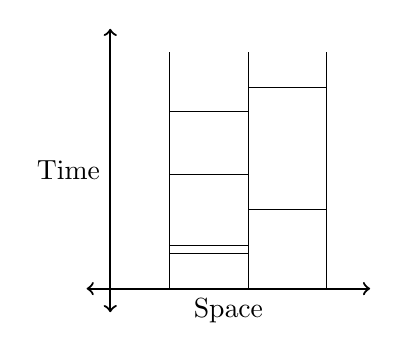
\begin{tikzpicture}
    \draw[<->,thick] (-0.3,0)--(3.3,0) node[midway,below] {Space};
    \draw[<->,thick] (0,-0.3)--(0,3.3) node[midway,left] {Time};
    \draw[-] (0.75,0)--(0.75,3);
    \draw[-] (1.75,0)--(1.75,3);
    \draw[-] (2.75,0)--(2.75,3);
    \draw[-] (0.75, 0.45)--(1.75, 0.45);
    \draw[-] (0.75, 0.55)--(1.75, 0.55);
    \draw[-] (0.75, 1.45)--(1.75, 1.45);
    \draw[-] (0.75, 2.25)--(1.75, 2.25);
    \draw[-] (1.75, 1)--(2.75, 1);
    \draw[-] (1.75, 2.55)--(2.75, 2.55);
\end{tikzpicture}
}\hspace{1in}
\subfloat[Locally Ordered]{
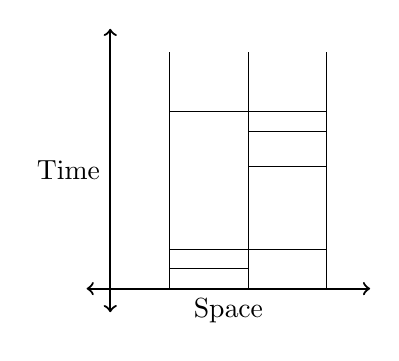
\begin{tikzpicture}
    \draw[<->,thick] (-0.3,0)--(3.3,0) node[midway,below] {Space};
    \draw[<->,thick] (0,-0.3)--(0,3.3) node[midway,left] {Time};
    \draw[-] (0.75,0)--(0.75,3);
    \draw[-] (1.75,0)--(1.75,3);
    \draw[-] (2.75,0)--(2.75,3);
    \draw[-] (0.75, 0.25)--(1.75, 0.25);
    \draw[-] (0.75, 0.5)--(1.75, 0.5);
    \draw[-] (0.75, 2.25)--(1.75, 2.25);
    \draw[-] (1.75, 0.5)--(2.75, 0.5);
    \draw[-] (1.75, 1.55)--(2.75, 1.55);
    \draw[-] (1.75, 2)--(2.75, 2);
    \draw[-] (1.75, 2.25)--(2.75, 2.25);
\end{tikzpicture}
}
\caption{Comparison of two event traces.}
\label{fig:sol-cartoon}
\end{figure}
Additionally, we define the value of an approximation at any point in time and space as the most recent average value of the cell containing the given point, i.e. 
\begin{equation*}
U(t,x) = \begin{cases}
U_j^n & \text{if } x \in (x_j, x_{j+1}) \quad \text{and} \quad t = t_{j^n},\\
U(\tprev_j, x) & \text{where } x \in (x_j, x_{j+1}).
\end{cases}
\end{equation*}
We also introduce $U_j(t)$ as the value of the solution $U(x,t)$ inside cell $j$ at time $t$. To approximate the flux exchange at the boundary, we define a numerical flux $\hat{F}(\cdot, \cdot)$. Additionally, we require that the numerical flux be:
\begin{enumerate}
\item {\em Consistent}, i.e. $\hat{F}(u^*,u^*) = f(u^*)$,
\item {\em Monotone}, i.e. $\hat{F}$ is increasing in the first argument, and decreasing in the second argument,
\item {\em Lipschitz continuous} in both arguments.
\end{enumerate}
We now define the Euler approximation to the scalar conservation law as follows.
\begin{definition}[Forward Euler Approximation]
An event trace $\mathcal{E}$ is an Euler approximation to the scalar conservation law if
\begin{equation}
U_j^{n+1} = U_{j}^n + \frac{1}{\Delta x_j}\int_{t_j^n}^{t_j^{n+1}} \big[ \hat{F}(U_{j-1}(\tau), U_j^n) - \hat{F}(U_j^n,U_{j+1}(\tau)) \big] \,\mathrm{d}\tau,
\label{eq:update}
\end{equation}
for all cells $j$, and between all updates $t_j^n$ and $t_j^{n+1}$, where $\hat{F}$ is a numerical flux.
\end{definition}

The remainder of this section assumes the existence of forward Euler approximations. Under this assumption, we present proofs that under CFL-like constraints, a maximum principle and total variation stability can be obtained. We note that the proofs follow closely the proof presented in~\cite{Osher1983,Kirby2003}. In the next section, we will present an algorithm which satisfies the assumptions of the theorems presented in this section.

Following the spirit of the analysis proposed in~\cite{Harten1983}, define
\begin{equation*}
C_j = - \left( \frac{ \hat{F}(U_j,U_{j+1}) - \hat{F}(U_{j-1},U_{j+1})}{\Delta x_j( U_j - U_{j-1})}\right) \text{ and } D_j = \frac{  \hat{F}(U_{j-1},U_{j+1}) - \hat{F}(U_{j-1},U_{j})}{\Delta x_j (U_{j+1} - U_{j})}.
\end{equation*}
We remark that due to the Lipschitz continuity of the numerical flux both $C_j$ and $D_j$ are bounded, and due to the monotonicity of the numerical flux $C_j \le 0 \le D_j$ for all $U_{j-1},U_j,U_{j+1}\in \mathbb{R}$. We reformulate the update rule \eqref{eq:update} as
\begin{equation}
U_j^{n+1} = U_j^n + \int_{t_j^n}^{t^{n+1}_j} \big[ C_j(\tau) \Delta U_{j-1}(\tau) - D_j(\tau) \Delta U_j(\tau) \big] \,\mathrm{d} \tau.
\label{eq:update2}
\end{equation}
Note that this representation is slightly different than the analyses presented in~\cite{Harten1983,Osher1983,Kirby2003}. We do not multiply our $C_j$ and $D_j$ coefficients by $\Delta t$.

\begin{theorem}[Maximum Principle]
Consider an event trace $\mathcal{E}$ satisfying the forward Euler approximation~\eqref{eq:update}. If given any two events $(t_j^n,\,U_j^n)$ and $(t_j^{n+1},\,U_j^{n+1})$,
\begin{equation}
1 + \int_{t_j^n}^{t_j^{n+1}} \big[ C_j(\tau) - D_j(\tau) \big] \,\mathrm{d}\tau \ge 0,
\label{eq:cfl-max}
\end{equation}
then
\begin{equation*}
|U^n_j| \le \sup_j |U^0_j|.
\end{equation*}
\label{thm:max}
\end{theorem}
\begin{proof}
Using the update criterion~\eqref{eq:update2},
\begin{equation*}
U^{n+1}_j = U_j^n + \int_{t_j^n}^{t_j^{n+1}} \big[ C_j(\tau) \Delta U_{j-1}(\tau) -D_j(\tau) \Delta U_j(\tau) \big] \, \mathrm{d}\tau
\end{equation*}
Using the CFL condition~\eqref{eq:cfl-max}, and $C_j(\tau) \le 0 \le D_j(\tau)$ for all $\tau$,
\begin{align*}
\left| U^{n+1}_j \right| & \le
\left| U_j^n + \int_{t^n_j}^{t^{n+1}_j} \big[ C_j(\tau) U_j^n - D_j(\tau)  U_j^n \big] \mathrm{d} \tau \right| \\
& \quad + \left| \int_{t^n_j}^{t^{n+1}_j} C_j(\tau) U_{j-1}(\tau) \mathrm{d} \tau \right| + \left| \int_{t^n_j}^{t^{n+1}_j} D_j(\tau) U_{j+1}(\tau) \mathrm{d} \tau \right|,\\
& \le \left( 1+ \int_{t^n_j}^{t^{n+1}_j} C_j(\tau)  + D_j(\tau) \, \mathrm{d} \tau \right) |U_j^n|\\
& \quad - \int_{t^n_j}^{t^{n+1}_j} C_j(\tau) |U_{j-1}(\tau)| \,\mathrm{d}\tau + \int_{t^n_j}^{t^{n+1}_j} D_j(\tau) |U_{j+1}(\tau)| \,\mathrm{d}\tau.
\end{align*}
Let $U^* = \sup_{\tau \in [t_j^n,t_j^{n+1})} \{ |U_j^n|, |U_{j-1}(\tau)|, |U_{j+1}(\tau)| \}$, then \
\begin{align*}
|U^{n+1}_j| & \le \left( 1 + \int_{t_j^n}^{t_j^{n+1}} \big[ C_j(\tau) - D_j(\tau) \big]\mathrm{d} \tau \right) U^* \\
& - \left(  \int_{t_j^n}^{t_j^{n+1}} C_j(\tau) \mathrm{d} \tau \right) U^* + \left(  \int_{t_j^n}^{t_j^{n+1}} D_j(\tau) \mathrm{d} \tau \right) U^*\\
& \le U^*.
\end{align*}

Lastly, we define the minimum time between events as
\begin{equation*}
\varepsilon = \inf_{j,k,n} \left\{ t_j^{n} - t \, : \, t \in \mathcal{T}_k \land t < t_j^n \right\}.
\end{equation*}
Since we've assumed a finite number of events, $\varepsilon>0$. Letting $\mathcal{U}(t)$ be defined as the largest value up till time $t$, i.e.
\begin{equation*}
\mathcal{U}(t) = \max_{j,\,\tau \le t} |U_j(\tau)|.
\end{equation*}
By the definition of $\varepsilon$, $U^* \le \mathcal{U}(t^{n+1}_j - \varepsilon/2)$.
Finally, we claim $\mathcal{U}((n+1)\varepsilon/2) \le \mathcal{U}(n\varepsilon/2)$. Pick any event at $t_i^m$ such that $n\varepsilon/2 < t_i^m \le (n+1) \varepsilon/2$. By the above analysis, 
\begin{equation*}
|U_i^m| \le \mathcal{U}(t_m^i - \varepsilon/2) \le \mathcal{U}(n\varepsilon/2).
\end{equation*}
Taking the maximum over all events occurring between $n\varepsilon/2$ and $(n+1)\varepsilon/2$, $\mathcal{U}((n+1) \varepsilon/2) \le \mathcal{U}(n \varepsilon)$. Arguing inductively, for all events $(t_j^n,\,U_j^n)$, $|U_j^n| \le \mathcal{U}(0) = \sup_j |U_j^0|$.
\end{proof}

\begin{remark}
This proof did not require that the solution be locally ordered.
\end{remark}

\subsection{TVD Analysis}
The main result of this section will be:
\begin{theorem}
\label{thm:tvd-stab}
A locally ordered forward Euler solution $\mathcal{E}$ subject to the following CFL constraint: for all cells $j$ and for all times between consecutive synchronization times, $t \in (s_{j,j+1}^{\mu}, s_{j,j+1}^{\mu+1})$,
\begin{equation}
1 + (\lceil t \rceil_{j+1} - s_{j,j+1}^{\mu})C_{j+1}(t) - (\lceil t \rceil_j - s_{j,j+1}^{\mu})D_{j}(t) \ge 0,
\label{eq:cfl-tvd}
\end{equation}
 is total variation diminishing (TVD), i.e.
\begin{equation*}
TV( U(t) ) = \sum_j |U_{j+1}(t) - U_j(t)| \le TV(U(0)).
\end{equation*}
\end{theorem}

\begin{remark}
The CFL condition presented here looks different than the one presented in Kirby~\cite{Kirby2003}. We've simply opted to use a less stringent inequality by making the time interval in the CFL condition span from the last synchronization time to the next update time rather than the next synchronization time.
\end{remark}
%\Max{Double check this remark}
Before we begin the proof, we introduce the following Lemma:
\begin{lemma}
\label{lem1}
Given cell $j$, and two update points, $t_1,\,t_2 \in \mathcal{T}_j$ and $t_1 < t_2$,
\begin{equation*}
\int_{t_1}^{t_2} \big[ U_j(t_1) - U_j(\tau) \big] \,\mathrm{d}\tau = - \int_{t_1}^{t_2} (t_2 - \lceil \tau \rceil_j) \big[ C_j \Delta U_{j-1}(\tau) + D_j \Delta U_j(\tau)\big] \,\mathrm{d} \tau.
\end{equation*}
\end{lemma}
\begin{proof}[Proof of Lemma \ref{lem1}]
Using the update relation,
\begin{equation*}
\int_{t_1}^{t_2} \big[ U_j(t_1) - U_j(\sigma) \big] \,\mathrm{d}\sigma = - \int_{t_1}^{t_2} \int_{t_1}^{\lfloor \sigma \rfloor_j} \big[ C_j \Delta U_{j-1}(\tau) + D_j \Delta U_j(\tau) \big] \,\mathrm{d} \tau \,\mathrm{d} \sigma.
\end{equation*}
Changing the order of integration, yields the result
\begin{align*}
\int_{t_1}^{t_2} \big[ U_j(t_1) - U_j(\sigma) \big] \,\mathrm{d}\sigma &= - \int_{t_1}^{t_2} \int_{\lceil \tau \rceil_j}^{t_2} \big[ C_j \Delta U_{j-1}(\tau) + D_j \Delta U_j(\tau) \big] \,\mathrm{d} \sigma \, \mathrm{d} \tau,\\
&= - \int_{t_1}^{t_2} (t_2 - \lceil \tau \rceil_j) \big[ C_j \Delta U_{j-1}(\tau) + D_j \Delta U_j ( \tau ) \big] \, \mathrm{d} \tau.
\end{align*}
\end{proof}


\begin{proof}[Proof of Theorem \ref{thm:tvd-stab}]
The proof closely follows that of~\cite{Kirby2003}. We've included it here for completeness.
Given an interface between cells $j$ and $j+1$ with consecutive synchronization times $\ssync$ and $\ssyncnext$, the update is given by
\begin{equation*}
\Delta U_j (\ssyncnext) = \Delta \left( U_j(\ssync) + \int_{\ssync}^{\ssyncnext} \big[ C_j \Delta U_{j-1} (\tau) + D_j \Delta U_{j} (\tau) \big] \,\mathrm{d} \tau \right)
\end{equation*}
Let $\Delta \ssync = \ssyncnext - \ssync$, we can then re-write the update rule as
\begin{align*}
\Delta U_j (\ssyncnext ) &= \frac{1}{\Delta \ssync} \bigg( \int_{\ssync}^{\ssyncnext} \Delta U_j(\ssync) - \Delta U_j(\tau) \,\mathrm{d} \tau \\
& + \Delta \int_{\ssync}^{\ssyncnext} U_j(\tau) + \Delta \ssync \big( C_j \Delta U_{j-1}(\tau) + D_j \Delta U_j(\tau) \big) \,\mathrm{d} \tau \bigg). \\
\end{align*}
By Lemma~\ref{lem1},
\begin{align*}
\Delta U_j (\ssyncnext ) &= \frac{1}{\Delta \ssync} \int_{\ssync}^{\ssyncnext} 
\Delta \left( U_j(\tau) +  (\lceil \tau \rceil_j - \ssync ) \left( C_j \Delta U_{j-1}(\tau) + D_j \Delta U_j(\tau) \right) \right)\,\mathrm{d} \tau\\
&= \frac{1}{\Delta \ssync} \int_{\ssync}^{\ssyncnext} \Big( 1 + ( \lceil \tau \rceil_{j+1} - \ssync ) C_{j+1}(\tau) - ( \lceil \tau \rceil_j - \ssync ) D_{j}(\tau) \Big) \Delta U_j(\tau) \,\mathrm{d} \tau\\
&\quad + \frac{1}{\Delta \ssync} \int_{\ssync}^{\ssyncnext} D_{j+1} \Delta U_{j+1}(\tau) - C_j \Delta U_{j-1} (\tau) \,\mathrm{d} \tau.
\end{align*}
Taking the absolute value of both sides, and using the CFL condition and $C_j \le 0 \le D_j$ for all $j$ and $\tau$, we obtain
\begin{multline}  \label{eq:thm1-pfa}
|\Delta U_j (\ssyncnext)| \le \frac{1}{\Delta \ssync} \int_{\ssync}^{\ssyncnext} \Big( 1 + ( \lceil \tau \rceil_{j+1} - \ssync ) C_{j+1}(\tau) - ( \lceil \tau \rceil_j - \ssync ) D_{j}(\tau) \Big) |\Delta U_j(\tau)| \,\mathrm{d} \tau\\
\quad + \frac{1}{\Delta \ssync} \int_{\ssync}^{\ssyncnext} ( \lceil \tau \rceil_{j+1} - \ssync )D_{j+1} |\Delta U_{j+1}(\tau)| - ( \lceil \tau \rceil_j - \ssync ) C_j |\Delta U_{j-1} (\tau)| \,\mathrm{d} \tau.
\end{multline}
Lastly, we establish bounds for $|\Delta U_j(\tau)|$. Consider the sequence of update points $\{t_k\}$ for either cell $j$ or $j+1$ in $[\ssync,\ssyncnext]$, i.e. $t_k \in \left(\mathcal{T}_j \cup \mathcal{T}_{j+1}\right) \cap [\ssync, \ssyncnext]$. Importantly, $\Delta U_j(\tau)$ is constant for all $\tau \in (t_k,t_{k+1})$. Then, for $r$, $t_{k+1} \le r < t_{k+2}$,
\begin{equation*}
\Delta U_j(r) = \Delta U_j(t_k) + \Delta \left( \int_{\lfloor t_k \rfloor_j }^{\lfloor r \rfloor_j} C_j \Delta U_{j-1}(\sigma) + D_j \Delta U_j(\sigma) \,\mathrm{d} \sigma \right).
\end{equation*}
Due to the local ordering constraint, either cell $j$ or cell $j+1$ will only update at $\ssync$ and $\ssyncnext$. Let us assume $\lfloor t_k \rfloor_j = \lfloor r \rfloor_j$. Taking the absolute value of both sides and grouping like terms, we obtain
\begin{align*}
|\Delta U_j(r)| &\le |\Delta U_j(t_k)| \left|1 + \int_{\lfloor t_k \rfloor_{j+1} }^{\lfloor r \rfloor_{j+1}} C_{j+1}(\sigma) \,\mathrm{d} \sigma \right| + \int_{\lfloor t_k \rfloor_{j+1} }^{\lfloor s \rfloor_{j+1}} D_{j+1}|\Delta U_{j+1}|(\sigma) \,\mathrm{d} \sigma.
\end{align*}
Using the CFL condition~\eqref{eq:cfl-tvd}, it follows that
\begin{equation*}
1 + \int_{\lfloor t_k \rfloor_{j+1}}^{\lfloor r \rfloor_{j+1}} C_{j+1}(\sigma) \,\mathrm{d}\sigma \ge 0.
\end{equation*}
%Let $\sigma^* = \argmin_{\sigma \in (\lfloor t_k \rfloor_{j+1}, \lfloor r \rfloor_{j+1})} C_j(\sigma)$. Then, noting that $\lfloor r \rfloor_{j+1} = t_{k+1} = \lceil \sigma^* \rceil_{j+1}$,
%\begin{align*}
%1 + \int_{\lfloor t_k \rfloor_{j+1} }^{\lfloor r \rfloor_{j+1}} C_{j+1}(\sigma) \,\mathrm{d} \sigma &\ge 
%1 + ( \lfloor r \rfloor_{j+1}- \lfloor t_k \rfloor_{j+1} ) C_{j+1}(\sigma^*)\\
%& \ge 1 + ( \lceil \sigma^* \rceil_{j+1} - \ssync ) C_{j+1}(\sigma^*)\\
%& \ge 0,
%\end{align*}
%by the CFL condition Equation \eqref{eq:cfl-tvd}. Note that the argument assuming $\lfloor r \rfloor_{j+1} = \lfloor t_k \rfloor_{j+1}$ follows similarly. %Therefore,
%\begin{align*}
%|\Delta U_j(r)| &\le |\Delta U_j(t_k)| + \int_{\lfloor t_k \rfloor_{j+1} }%^{\lfloor s \rfloor_{j+1}} C_{j+1} |\Delta U_j|(\sigma) + D_{j+1} |\Delta U_{j-1}|(\sigma) \,\mathrm{d} \sigma \\
%&\quad - \int_{\lfloor t_k \rfloor_{j} }^{\lfloor s \rfloor_{j}} C_{j} |\Delta U_{j-1}|(\sigma) + D_{j} |\Delta U_{j}|(\sigma) \,\mathrm{d} \sigma.
%\end{align*}
Summing over the update points $\{t_k\}$, for $r < \ssyncnext$, we obtain
\begin{align*}
|\Delta U_j(r)| &\le |\Delta U_j(\ssync)| + \int_{ \ssync }^{\lfloor r \rfloor_{j+1}} C_{j+1} |\Delta U_j|(\sigma) + D_{j+1} |\Delta U_{j+1}|(\sigma) \,\mathrm{d} \sigma \\
&\quad - \int_{ \ssync }^{\lfloor r \rfloor_{j}} C_{j} |\Delta U_{j-1}|(\sigma) + D_{j} |\Delta U_{j}|(\sigma) \,\mathrm{d} \sigma.
\end{align*}
Substituting this expression into \eqref{eq:thm1-pfa},
\begin{align*}
|\Delta U_j ( \ssyncnext)| & \le | \Delta U_j(\ssync)|\\
& \quad + \frac{1}{\Delta \ssync} \int_{\ssync}^{\ssyncnext} ( \lceil \tau \rceil_{j+1} - \ssync ) \left( C_{j+1} |\Delta U_j|(\tau) + D_{j+1} | \Delta U_{j+1}| (\tau) \right) \,\mathrm{d} \tau\\
& \quad - \frac{1}{\Delta \ssync} \int_{\ssync}^{\ssyncnext} ( \lceil \tau \rceil_{j} - \ssync ) \left( C_{j} |\Delta U_{j-1}|(\tau) + D_{j} | \Delta U_{j}| (\tau) \right) \,\mathrm{d} \tau\\
& \quad + \frac{1}{\Delta \ssync} \int_{\ssync}^{\ssyncnext} \int_{\ssync}^{\lfloor \tau \rfloor_{j+1}}C_{j+1} |\Delta U_j|(\sigma) + D_{j+1} | \Delta U_{j+1}| (\sigma)\,\mathrm{d} \sigma \,\mathrm{d} \tau\\
& \quad - \frac{1}{\Delta \ssync} \int_{\ssync}^{\ssyncnext}\int_{\ssync}^{\lfloor \tau \rfloor_{j}} C_{j} |\Delta U_{j-1}|(\sigma) + D_{j} | \Delta U_{j}| (\sigma) \,\mathrm{d} \sigma\,\mathrm{d} \tau\\
\end{align*}
Reversing the order of integration for the double integrals, we obtain
\begin{align*}
|\Delta U_j (\ssyncnext)| & \le | \Delta U_j(\ssync)|\\
& \quad + \frac{1}{\Delta \ssync} \int_{\ssync}^{\ssyncnext} ( \lceil \tau \rceil_{j+1} - \ssync ) \left( C_{j+1} |\Delta U_j|(\tau) + D_{j+1} | \Delta U_{j+1}| (\tau) \right) \,\mathrm{d} \tau\\
& \quad - \frac{1}{\ssync} \int_{\ssync}^{\ssyncnext} ( \lceil \tau \rceil_{j} - \ssync ) \left( C_{j} |\Delta U_{j-1}|(\tau) + D_{j} | \Delta U_{j}| (\tau) \right) \,\mathrm{d} \tau\\
& \quad + \frac{1}{\Delta \ssync} \int_{\ssync}^{\ssyncnext} ( \ssyncnext - \lceil \tau \rceil_{j+1} ) \left( C_{j+1} |\Delta U_j|(\tau) + D_{j+1} | \Delta U_{j+1}| (\tau) \right) \,\mathrm{d} \tau\\
& \quad - \frac{1}{\Delta \ssync} \int_{\ssync}^{\ssyncnext} ( \ssyncnext - \lceil \tau \rceil_{j}) \left( C_{j} |\Delta U_{j-1}|(\tau) + D_{j} | \Delta U_{j}| (\tau) \right) \,\mathrm{d} \tau\\
& = | \Delta U_j(\ssync)|\\
& \quad + \int_{\ssync}^{\ssyncnext} C_{j+1} |\Delta U_j|(\tau) + D_{j+1} | \Delta U_{j+1}| (\tau) \,\mathrm{d} \tau\\
& \quad - \int_{\ssync}^{\ssyncnext} C_{j} |\Delta U_{j-1}|(\tau) + D_{j} | \Delta U_{j}| (\tau) \,\mathrm{d} \tau\\
\end{align*}
Summing over all synchronization times, we obtain
\begin{equation*}
|\Delta U_j (t)| \le |\Delta U_j(0)| + \Delta \int_0^t C_j |\Delta U_{j-1}| + D_j |\Delta U_j|\,\mathrm{d} \tau.
\end{equation*}
Summing across all cells $j$ gives the result.
\end{proof}
 %3 pages

% This file contains lst listing snippets which are necessary to embed the lstlistings into subfloats
% https://tex.stackexchange.com/a/34951

\newsavebox{\submeshlisting}
\begin{lrbox}{\submeshlisting}
\begin{lstlisting}[mathescape=true,basicstyle=\scriptsize]
class Submesh
  $id \in \mathbb{Z}$
  $t,\,\tprev,\,\tnext\in \mathbb{Z}$
  $u,\,\Delta x \in \mathbb{R}^{n_{el}}$
  $\ell,\,r \in$ Interface
\end{lstlisting}
\end{lrbox}


\newsavebox{\interfacelisting}
\begin{lrbox}{\interfacelisting}
\begin{lstlisting}[mathescape=true,basicstyle=\scriptsize]
class Interface
  $id \in \mathbb{Z}$
  $\tprev,\,\tsync \in \mathbb{Z}$
  $u,\,\Sigma \hat{F},\,\Delta x \in \mathbb{R}$
  $K^{int},\,K^{ext} \in \mathbb{R}$
\end{lstlisting}
\end{lrbox}

\section{An Adaptive Local Timestepping Algorithm}
\label{sec:alg}
The previous proofs dealt with certain classes of event traces and demonstrated that they were TVD. In this section, we present an algorithm that generates an event trace satisfying the hypotheses of Theorem \ref{thm:tvd-stab}. To allow for an efficient implementation, we couch the algorithm in the language of discrete event simulations, which will allow us to rely on the extensive work done in that field for the parallelization. The main result of this section will demonstrate that with a sufficiently small minimum timestep, our algorithm will generate a total variation stable event trace.

\subsection{Discrete Event Simulation}
Discrete event simulation as a tool has been used extensively for the simulation of numerous phenomena~\cite{Fujimoto1990}. Fundamentally, the simulation is represented as a set of actors denoted here as $\mathcal{A}$, and a set of events to be executed on an actor at a given point in time. When executed, each event may then schedule more events with later timestamps. The discrete event simulator guarantees that events will be executed in order of their timestamps.
%\Cy{It's probably worth mentioning here that we use sub-times to schedule multiple events at the same $\tau$ timestamp.}

At a high level, the actors used for the approximation of solutions to conservation laws will consist of submeshes. For this section, we require that at least two elements be assigned to each submesh. However, given an update rule with a $2n+1$-sized stencil per cell as is the case for high order finite volume methods, we require that the submesh contain at least $n+1$ cells. In practice, achieving performance requires balancing the overhead of the simulator against the amount of useful work being done during each task~\cite{Bremer2019}. Therefore, submeshes should contain significantly more cells to balance simulation overheads. Each submesh can schedule one of two events: (1) {\em Update} ($\mathcal{U}$) the submesh to the time at which the update is scheduled, and (2) {\em Push Flux} ($\mathcal{PF}$), wherein the submesh sends relevant metadata to the neighboring cell to allow advancing along the shared boundary. We quantize our time to be an integer multiple of a smallest timestep, $\Delta t_{\min}$. In this section, we use $t,\,\tprev,\,\tnext$ as variable names and $\tau$ is used to specify timestamps in the discrete event simulation.

\begin{figure}
\centering
\subfloat[Submesh class\label{class:submesh}]{\usebox{\submeshlisting}}\hspace{2in}
\subfloat[Interface class\label{class:interface}]{\usebox{\interfacelisting}}
\caption{Local timestepping data structures}
\end{figure}

The actor states are described in Figure~\ref{class:submesh}. The actor's members correspond to
\begin{itemize}
\item $id$: The submesh id,
\item $t$: The current time of the submesh,
\item $\tprev$: The last time at which the submesh was updated,
\item $\tnext$: The next time at which the submesh is scheduled to be updated,
\item $u$: The average density on each cell,
\item $\Delta x$: The sizes of the cells for the submesh,
\item $\ell,\,r$: Representations of the states to the left and right of the submesh, respectively. 
\end{itemize}
The interface class in Figure~\ref{class:interface} describes neighboring cell metadata and has members describing: %\Max{Description of K confusing} %\Cy{Consider using a different symbol for the $\tprev$ in the interface vs the $\tprev$ in the actor}
\begin{itemize}
\item $id$: The id of the neighboring submesh,
\item $\tprev$: The last time at which the neighbor was updated,
\item $\tsync$: The last time at which the neighbor and submesh both updated,
\item $u$: The neighbor's density at time $\tprev$,
\item $K^*$: The largest Lipschitz constant of the numerical flux between time $\tsync$ to $\tprev$ on the internal interface ($K^{\intr}$) or external interface cell ($K^{\extr}$),
\item $\Sigma \hat{F}$: The integral of the numerical flux between the submesh and its neighbor from time $\tprev$ to the current time,
\item $\Delta x$: is the size of the neighboring cell.
\end{itemize}
We note that the Lipschitz constant $K$ is used to bound $C_j$ and $D_j$ terms simultaneously. For commonly used fluxes like the Godunov flux or Lax-Friedrichs flux, $K$ will look like $|\Lambda|/\Delta x$ yielding the commonly seen version of the CFL condition \eqref{eq:vanilla-cfl}.
Member fields are denoted using a period, e.g. $S.\ell.\tprev$ denotes the previous update of the left interface of submesh $S$.
We next turn to describing our events. Before we define our two main events, {\sc update} and {\sc push\_flux}, we define some helper functions.
\begin{definition}[Helper Functions]
\label{def:helper-functions}
\begin{itemize}
\item {\sc advance(t, submesh)}: Advance the submesh one timestep from submesh.$\tprev$ to $t$ according to the update rule~\eqref{eq:update}. Note that this will also cause corresponding updates in boundary terms such as $K^*$ and $\Sigma \hat{F}$.
\item {\sc compute\_t\_next\_bdry(submesh, neigh)}: Compute the timestep size for interfaces which depend on neigh.$u$. This evaluates two CFL conditions at: (1) the external interface between the submesh and its neighbor, which is synchronized at neigh.$\tsync$ and (2) the internal interface nearest to the external interface, which is synchronized at submesh.$\tprev$.
\item {\sc compute\_t\_next(submesh, t)}: Compute the allowable timestep size for the submesh. This is taken to be the minimum of the largest timesteps for the values returned by {\sc compute\_t\_next\_bdry} for both neighbors and the largest allowable internal timestep.
\item {\sc make\_msg(submesh, neigh)}: Generate a buffer with the required information to update the neighbor's corresponding interface.
\item {\sc accumulate(t, submesh, neigh)}: Update neigh.$\Sigma \hat{F}$ to integrate from the previous integration point neigh.$\tprev$ to time $t$. 
\item {\sc update\_K\_bdry(submesh, neigh)}: Update Lipschitz constants $K^*$ according to the new updated values at the boundary.
\end{itemize}
\end{definition}
The helper functions serve as an API between the application and the timestepping algorithm. Features like which set of conservation laws or choice of discretization are encapsulated into the above function calls. In addition to the helper functions, we also define our scheduling primitives. These are the function calls with which events are scheduled in the discrete event simulator.

\begin{definition}[Scheduling Primitives]
\label{def:scheduling-primitives}
\begin{itemize}
\item {\sc schedule(t, event)}: Schedule {\sc event} at time {\sc t} in the discrete event simulator.
\item {\sc schedule\_inline(event)}: Execute {\sc event} in the current execution context, i.e. on that actor at that time.
\end{itemize}
\end{definition}

\begin{figure}
\begin{lstlisting}[mathescape=true, basicstyle=\scriptsize]
function update(id, update_forced)
  $\tau \gets$ get_time()
  submesh $\gets$ get_submesh(id)

  if ( $\tau \neq \text{submesh}.\tnext \land \neg \text{force\_update}$ ) return
  if ( $\tau = \text{submesh}.\tprev$ ) return
    
  advance($\tau$, submesh)
  submesh.$\tnext$ $\gets$ compute_t_next(submesh, $\tau$)
  
  for neigh $\in$ submesh.bdry
    forced_update $\gets$ neigh.$\tprev$ > neigh.$\tsync$
                  $\land$ compute_t_next_bdry(submesh, neigh) $\le \tau$
                  
    schedule( $\tau$, push_flux( neigh.id, id,
                            make_msg(submesh, neigh),
                            force_update) )
    if ( forced_update ) neigh.$\tsync$ $\gets\tau$
    
  if ( submesh.$\tnext > \tau$ )
    schedule(submesh.$\tprev$, update(id, false))
\end{lstlisting}
\caption{Update function}
\end{figure}

\begin{figure}
\begin{lstlisting}[mathescape=true,basicstyle=\scriptsize]
function push_flux(id, id_from, msg, force_update)
  $\tau \gets$ get_time()
  submesh $\gets$ get_submesh(id)
  neigh $\gets$ get_neigh(submesh, id_from)
  
  accumulate( $\tau$, submesh, neigh )
  neigh.u $\gets$ msg
  neigh.$\tprev$ $\gets \tau$
  if ( neigh.$\tprev =$submesh.$\tprev$ ) neigh.$\tsync$ $\gets \tau$
  update_K_bdry(submesh, neigh)
  
  submesh.$\tnext$ $\gets$ compute_t_next(submesh, $\tau$)
  if ( force_update $\lor$ submesh.$\tnext \le \tau$ )
    schedule_inline(update(id, true))
    return
    
  if ( submesh.$\tnext > \tau$ )
    schedule(submesh.$\tnext$, update(id, false))
\end{lstlisting}
\caption{Push flux function}
\end{figure}

With these helper functions, we now define our two main events: update ($\update$) and push flux ($\pushflux$). Shown in Algorithm~\ref{alg:des}, the main loop schedules initial updates at time 0 in a priority queue ($\pq$). As events execute, they may cause other events to be enqueued in the priority queue as pairs with the desired timestamp of evaluation as the key. The lowest timestamps receive the highest priority, and in case of ties, we impose no ordering.

\begin{algorithm}
\caption{Main timestepping loop}\label{alg:des}
\begin{algorithmic}
\State Initialize actors $\mathcal{A}= \{ S_1,\ldots, S_{n_{sbmsh}} \}$
\State Initialize $\pq := \{\}$
\For{$sbmsh \in \mathcal{A}$}
  \State schedule( 0, update($sbmsh.id$, false))
\EndFor

\While{$\exists\,q \in \pq$}
  \State current\_event $\gets \pq$.pull\_highest\_priority()
  \State evaluate(current\_event)
\EndWhile
\end{algorithmic}
\end{algorithm}

We now arrive at the main result for this section.
\begin{theorem}
\label{thm:des-tvd}
Given a minimum timestep size of
\begin{equation}
\Delta t_{\min} < \inf\left\{ \frac{\Delta x_{\min}}{2 \max(K_1(\xi),\,K_2(\xi))}\, : \, \xi \in \range(u_0) \right\},
\label{eq:dt-min}
\end{equation}
where $\Delta x_{\min}$ is the smallest element size, $K_1(\xi)$ is the local Lipschitz constant of $\hat{F}(\cdot,\xi)$ and $K_2(\xi)$ is the local Lipschitz constant of $\hat{F}(\xi,\cdot)$. The discrete event simulator as defined in Algorithm \ref{alg:des} with a minimum timestep of $\Delta t_{\min}$ will produce a TVD solution to the scalar conservation law in~\eqref{eq:ivp}.
\end{theorem}

\subsection{Proof of Theorem \ref{thm:des-tvd}}
The proof of the theorem requires demonstrating that the discrete event simulation generates an event trace that satisfies the conditions of Theorem~\ref{thm:tvd-stab}. The main machinery for this proof will be loop invariants. Loop invariants are a formal correctness technique whereby we specify a set of ``correct'' states. By showing that every event maps a correct state onto the set of correct states, we are able to ensure that the following state satisfies certain desired criteria. Once all events have executed, we will have proven that the simulation terminates in the correct state and the algorithm behaves as desired. This proof technique has been utilized with great success for systematic design of algorithms for numerical linear algebra as part of the FLAME project~\cite{Bientinesi2011, Myers2018}.
 To demonstrate that the algorithm satisfies the conditions of Theorem~\ref{thm:tvd-stab}, we need invariants to satisfy:
\begin{enumerate}
\item the local ordering principle,
\item the CFL condition,
\item and the update rule as expressed in \eqref{eq:update}.
\end{enumerate}
Additionally, we will require two further invariants to show that the computed values are correct, and that duplicated metadata in the boundaries is consistent with the values on the neighboring submesh. To simplify, the notation in these invariants, we assume three submeshes are enumerated as, $S_A$, $S_B$, and $S_C$. The value of $u$ at the cell neighboring another submesh, will be indexed with that neighbors name, e.g. the cell in submesh $S_B$ that neighbors $S_A$ we will reference as $S_B.u_A$. For clarity, we have depicted this naming convention in Figure~\ref{fig:submeshes}.
\begin{figure}
\centering
  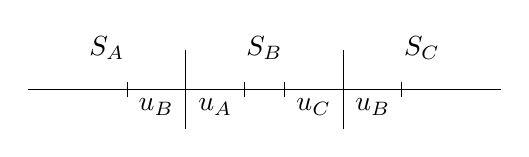
\begin{tikzpicture}
    \draw (-3,0)-- (-1,0) node[midway, above, label={[distance=1cm]:$S_A$}] {};
    \draw (-1,0)-- ( 1,0) node[midway, above, label={[distance=1cm]:$S_B$}] {};
    \draw ( 1,0)-- ( 3,0) node[midway, above, label={[distance=1cm]:$S_C$}] {};
    \draw (-1,-0.5)--(-1,0.5);
    \draw ( 1,-0.5)--( 1,0.5);
    \draw[|-] (-1.75,0)--(-1,0) node[midway,below] {$u_B$};
    \draw[-|] (-1,0)--(-0.25,0) node[midway,below] {$u_A$};
    \draw[|-] ( 0.25,0)--( 1,0) node[midway,below] {$u_C$};
    \draw[-|] ( 1,0)--( 1.75,0) node[midway,below] {$u_B$};
  \end{tikzpicture}
\caption{Three neighboring submeshes $S_A,\,S_B,$ and $S_C$ with bordering cells named.}
\label{fig:submeshes}
\end{figure}
% \Cy{consider more clearly defining the term "synchronization time" at or before this point}\Max{This is introduced in the first order method section.}


Local ordering implies that one of two neighboring submeshes must have last updated at the last synchronization time.  To ensure that the event trace will be locally ordered, we define the local ordering invariant for the left interface as
\begin{align}
LO_{\ell}(S_B,\tau) &= (S_B.\tprev = S_B.\ell.\tsync\,\lor\,S_B.\ell.\tprev = S_B.\ell.\tsync) \label{eq:LO1}
\end{align}
%\Cy{This is the first use of $\tau$ I found in this section.  I think I figured it out: $\tau$ is just a particular time you're evaluating the invariants, and the various $t$s are used as variable names.}
Note that we similarly define $LO_r(S_B,\tau)$ for the right interface. The $\tau$ in the arguments of the loop invariants refers to the simulation time at which we evaluate the invariant.

Next, we define the CFL-related invariants. These invariants will ensure that our algorithm satisfies the CFL condition~\eqref{eq:cfl-tvd}. Define the invariant for the left boundary cell as
\begin{align}
CFL_{\ell}(S_B, \tau) &= ( S_B.\tnext - S_B.\ell.\tsync) S_B.\ell.K^{\extr} \le 1/2 \label{eq:CFL:ext}\\
& \land\, (S_B.\tnext - S_B.\tprev) S_B.\ell.K^{\intr} \le 1/2, \label{eq:CFL:int}
\end{align}
where $K$ is used to bound the respective $C_j$ and $D_j$ terms. Note that \eqref{eq:CFL:ext} corresponds to interface between submeshes $S_A$ and $S_B$, thus the CFL condition is relative to $S_B.\ell.\tsync$. The other CFL condition \eqref{eq:CFL:int} corresponds to the interior interface of the cell associated with $S_B.u_a$. Since internally the internal cells step synchronously, the last synchronization time is $S_B.\tprev$, but since $S_B.\ell.K^{\intr}$ still depends on $S_B.\ell.u$, this condition must be re-evaluated after each push flux. We  define a CFL invariant for the right interface, $CFL_r(S_B, \tau)$ similarly. We also define an internal CFL invariant, $CFL_{\intr}$, which can be determined by solely examining the internal state of the submesh.
\begin{equation*}
    CFL_{\intr} = \bigwedge_{i=2}^{n_{el-1}} \big( (S_B.\tnext - S_B.\tprev) \big[D_i(S_B.u_{i-1},S_B.u_i, S_B.u_{i+1}) - C_i(S_B.u_{i-1},S_B.u_i,S_B.u_{i+1})\big] \le 1 \big)
\end{equation*}
We then define our CFL invariant as
\begin{equation}
CFL(S_B,\tau) =  (CFL_{\intr}\,\land\,CFL_{\ell}\,\land\,CFL_r). \label{eq:CFL:1}
\end{equation}
The correctness invariant $CR$ checks that all computations are being done correctly. Here, we use $\tilde{S}_B$ to denote the state before executing an event.
\begin{align}
CR&(S_B,\tau) = \big( (S_B.\tprev =\tilde{S}_B.\tprev\,\land\,S_B.u = \tilde{S}_B.u) \label{eq:CR1}\\
&\quad\quad\lor (S_B.\tprev \neq \tilde{S}_B.\tprev \,\land\,S_B\text{ updated according to Equation~\eqref{eq:update}} \big)\label{eq:CR2}\\
&\land \left( S_B.\ell.\Sigma \hat{F} = \int_{S_B.\tprev}^{\max(S_B.\ell.\tprev,S_B.\tprev)} \hat{F}(S_B.\ell.u(\sigma), S_B.u_A) \,\mathrm{d}\sigma \right)\label{eq:CR3}\\
&\land \left( S_B.r.\Sigma \hat{F} = \int_{S_B.\tprev}^{\max(S_B.r.\tprev,S_B.\tprev)} \hat{F}(S_B.u_C, S_B.r.u(\sigma)) \,\mathrm{d}\sigma \right)\label{eq:CR4}\\
& \land\,S_B.\ell.K^{\intr} \ge \max_{\sigma \in (S_B.\tprev, \tau)} D_j(S_B.\ell.u(\sigma), S_B.u_A, S_B.u_{A+1})\label{eq:CR5}\\
& \land\,S_B.\ell.K^{\extr} \ge \max_{\sigma \in (S_B.\ell.\tsync, \tau)} -C_j(S_B.\ell.u(\sigma), S_B.u_A, S_B.u_{A+1})\label{eq:CR6}\\
& \land\,S_B.r.K^{\intr} \ge \max_{\sigma \in (S_B.\tprev, \tau)} -C_j(S_B.u_{C-1}, S_B.u_C, S_B.r.u(\sigma))\label{eq:CR7}\\
& \land\,S_B.r.K^{\extr} \ge \max_{\sigma \in (S_B.r.\tsync, \tau)} D_j(S_B.u_{C-1}, S_B.u_C, S_B.\ell.u(\sigma)).\label{eq:CR8}
\end{align}
%\Cy{In (4.13) to (4.16), some $u$ values are not dependent on $\sigma$ because their values are constant over the interval, right?  The reader will probably notice this, but I'm not sure if this is worth mentioning in the text.}
 Equations~\eqref{eq:CR1} and~\eqref{eq:CR2} require that if the state has been updated, $S_B.\tprev$ will reflect that, and that the state is updated according to the update rule. We check that the flux buffers are being correctly integrated at the boundary with \eqref{eq:CR3} and~\eqref{eq:CR4}. The last set of equations \eqref{eq:CR5}--\eqref{eq:CR8} check that the $K$ terms used to enforced the CFL condition correctly bound the Lipschitz constants of the numerical flux. Internal values of $S_B.u$ in \eqref{eq:CR5}--\eqref{eq:CR8} have no dependence on the time variable $\sigma$ since the solution remains constant on a cell between updates. For this invariant to be well-defined, we require that each submesh contain at least two cells. Otherwise, terms like $S_B.u_{A+1}$ would not exist.

The previous three invariants, $LO, CFL,$ and $CR$, have all used information available on submesh $S_B$. However, when duplicating information between neighbors, we need to ensure that the information is consistent. Thus, we define a consistency invariant,
\begin{align}
CI(S_B, S_A, \tau) &= \big( S_B.u_A = S_A.r.u_B \,\land\, S_B.\tprev = S_A.r.\tprev)\label{eq:CI1}\\
&\quad\quad \lor\, \exists\,(\tau,\pushflux(S_A.id, S_B.id, S_B.u_a, \cdot))
\in\pq \big)\label{eq:CI2}\\
&\land\,\big( S_B.\ell.\tsync = S_A.r.\tsync\label{eq:CI3}\\
&\quad \lor\, ( S_B.\ell.\tsync = \tau \,\land\,\exists\,(\tau,\pushflux(S_A.id,S_B.id,\cdot,\cdot))\in \pq\label{eq:CI4}\\
&\quad\lor\, (S_A.r.\tsync=\tau \,\land\,\exists\,(\tau,\pushflux(S_B.id,S_A.id, \cdot, \cdot)) \in \pq \big)\label{eq:CI5}
\end{align}
Here we use the dot, $\cdot$ to denote any argument. Note that we similarly define consistency for the other interface between $S_B$ and $S_C$.

The last invariant we define is a progress invariant to ensure that the simulation can make progress,
\begin{align}
P(S_B, \tau) &= (S_B.\tprev = t_{end})\\
&\lor  (\exists\,(s,\update(s,S_B,false))\in\pq \, :\, \{s = \,S_B.\tnext \ge \tau > S_B.\tprev\})\label{eq:P2}\\
&\lor  \exists\,(\tau, \pushflux(S_B.id, \cdot, \cdot,\cdot))\in \pq \label{eq:P3} \\
&\lor  \exists\,(\tau, \pushflux(\cdot, S_B.id, \cdot, true))\in\pq. \label{eq:P4}
\end{align}
Combining these five loop invariants, we arrive at
\begin{align}
I(S_B, S_A, S_C, \tau) &= LO_{\ell}(S_B) \,\land\, LO_r(S_B) \,\land\,CFL(S_B, \tau) \land CR(S_B, \tau)\\
&\land\,CI(S_B,S_A, \tau) \,\land\, CI(S_B,S_C,\tau)\,\land P(S_B,\tau).
\end{align}

As the aim is to ensure the invariants hold for all submeshes, we will refer to $I(\tau)$ (without the submesh arguments) as
\begin{equation*}
I(\tau) = \bigwedge_{k=1}^{\nsbmsh} I(S_k, S_{k-1}, S_{k+1}, \tau).
\end{equation*}
\begin{proposition}
A discrete event simulation which satisfies the invariant $I$ between all events executed before time $\tau$, will execute a finite number of events at $\tau$ and satisfy $I$ between each of these events.
\label{prop:1step}
\end{proposition}
Assuming Proposition~\ref{prop:1step} holds, the remainder of the proof of Theorem~\ref{thm:des-tvd} follows by induction. At the start of time $\tau$ , we note that no updates have executed, and so $S.\tprev < \tau$. Furthermore, since push fluxes may only be scheduled at the time at which the spawning updates are executed, there are no outstanding push fluxes. Thus, the invariant $I$ before any events have been executed at time $\tau$ is
%\Cy{This might also be a good point to discuss sub-times since we have multiple events executing at a single timestamp.}
%\Cy{use "time" vs "timestamp" consistently}
\begin{align*}
I(\tau, S_B, S_A, S_C) &= LO_{\ell} \,\land\,LO_r\,\land\,CFL_{\intr} \,\land\,CFL_{\ell}\,\land\,CFL_r\,\land\,CR\\
&\land\,S_B.u_A = S_A.r.u_B \,\land\,S_B.\tprev = S_A.r.\tprev\\
&\land\,S_B.\ell.\tsync = S_A.r.\tsync\\
&\land\,S_B.u_C=S_C.\ell.u_B\,\land\,S_B.\tprev =S_C.\ell.\tprev\\
&\land\,S_B.r.\tsync = S_C.\ell.\tsync\\
&\land\,\exists\,(s,\mathcal{U}(S_B.id, false)) \in \mathcal{Q} \text{ for which } \tau \le s \le S_B.\tnext.
\end{align*}
After all events at time $\tau$ have finished executing, we end in the same state, with the exception that the progress invariant implies that every element must have an update scheduled at a time strictly greater than $\tau$. Due to consistency and correctness, every cell which updated at time $\tau$, was updated according to the update rule \eqref{eq:update}. Furthermore, consistency and correctness along with the CFL condition, imply that the event trace up until time $\tau$ satisfies the CFL condition~\eqref{eq:cfl-tvd}. Once all the events have executed, remaining in $I$ implies that updates must be scheduled for time $\tau+\Delta t_{\min}$ or greater, since otherwise the discrete event simulation would not advance past time $\tau$ in a finite number of events. Lastly, the event trace remains locally ordered. Were it not, one of the locally ordered invariants would be violated after all events at $\tau$ had executed. Remarking that the solution remains constant from $\tau$ to $\tau + \Delta t_{\min}$, we have established the inductive hypothesis. Arguing inductively, the event trace at $\tend$ is locally ordered, satisfies the CFL condition, and obeys the forward Euler update rule. Therefore, the discrete event simulation will generate a TVD solution.
%\Cy{$\tau + \Delta t_{\min}$?  I'm still not sure if $\tau$ is in units of seconds or $\Delta t_{\min}$ increments} \Max{Should be \tau + \Delta t_{\min}}


\subsection{Proof of Proposition \ref{prop:1step}}
The remainder of the proof relies on demonstrating that the simulation state satisfies the invariants after each event is evaluated at time $\tau$. However, before we proceed, we prove a progress guarantee.

\begin{proposition}
Given a discrete event simulation that satisfies invariant $I$ up until time $\tau$, $u(\tau)$ will satisfy a maximum principle.
\label{prop:des-max}
\end{proposition}
\begin{proof}
Pick any cell $j$ and consider two update points $t_j^n$ and $t_j^{n+1}$. Let $s_{j-1,j}^{\mu}$ and $s_{j,j+1}^{\eta}$ represent the most recent left and right synchronization times, respectively, and let $u_{j-1}$, $u_j$, $u_{j+1}$ represent the associated cell densities.
Since the total variation CFL condition~\eqref{eq:cfl-tvd} is satisfied for all time up until $\tau$,
\begin{align*}
1 &+ \int_{t_j^n}^{t_j^{n+1}} \big[C_j(\sigma) - D_j(\sigma) \big]\,\mathrm{d} \sigma\\
& \ge 1 + (t_j^{n+1} - s_{j-1,j}^{\mu}) \min_{\sigma \in (s_{j-1,j}^{\mu},t_j^{n+1})} C_j(u_{j-1}, u_j, u_{j+1})\\
& \quad\quad - (t_j^{n+1} - s_{j,j+1}^{\eta}) \max_{\sigma \in (s_{j,j+1}^{\eta}, t_j^{n+1})}D_j(u_{j-1}, u_j, u_{j+1})\\
& \ge 0.
\end{align*}
Thus, the event trace satisfies the maximum principle, Theorem~\ref{thm:max}.
\end{proof}

\begin{lemma}[Progress Guarantees]
\label{lem:progress-guarantee}
Given a simulation that satisfies the invariant $I$ up until time $\tau$, if a submesh $S_B$ and its neighbors $S_A$ and $S_B$ are both updated at time $\tau$, then
\begin{lstlisting}[mathescape=true]
    compute_t_next(submesh, $\tau$) $\ge \tau + \Delta t_{\min}$.
\end{lstlisting}
\end{lemma}
\begin{proof}
Pick any cell of $S_B$ and consider the two neighboring cells. Enumerate the densities as $u_{j-1},\,u_j$ and $u_{j+1}$. 
By definition of the Lipschitz constant
\begin{equation*}
-C_j(u_{j-1}, u_j, u_{j+1}) \le K_1(u_{j+1})/\Delta x_{\min}
\end{equation*}
for all $u_{j-1},\,u_j,\,u_{j+1} \in \range(u_0)$.
By Proposition \ref{prop:des-max}, $u_{j-1}, u_j, u_{j+1} \in \range(u_0)$. Therefore,
\begin{align*}
-\Delta t_{\min} C_j(u_{j-1}, u_j, u_{j+1}) \le \frac{K_1(u_{j+1})}{\Delta x_{\min}} \frac{\Delta x_{\min}}{2K_1(u_{j+1})} = \frac{1}{2}
\end{align*}
The proof for the right interface of cell $j$ follows similarly. Thus, taking a timestep of size $\Delta t_{\min}$ satisfies~\eqref{eq:cfl-tvd}.
Since this holds for every cell in submesh $S_B$,
\begin{lstlisting}[mathescape=true]
get_t_next(submesh, $\tau$) $\ge \tau + \Delta t_{\min}$.
\end{lstlisting}
\end{proof}

To see that there are at most a finite number of messages sent at each $\tau$, note that each update will only execute the main body at most once for a given timestep. If multiple updates are scheduled for the same time $\tau$, $S_B.\tprev = \tau$ after the first update, and subsequent update events would cause the function to become a no-op. Furthermore, since push fluxes can only be scheduled when an update has executed at that timestep, we bound the total number of events scheduled at a given timestep by $3 \nsbmsh$.

Completing the proof requires showing that as each event at time $\tau$ is processed $I$ is not violated. To do so, we will enumerate some states of the submesh and show that execution of any event will not lead to an invariant violation. In order to determine the state of a submesh $S$, we require 6 Boolean variables:
\begin{align*}
b_1 &= (S.\tprev < \tau)\\
b_2 &= (S.\tnext > \tau)\\
b_3 &= (S.\ell.\tprev < \tau)\\
b_4 &= (S.\ell.\tsync \le S.\ell.\tprev)\\
b_5 &= (S.r.\tprev < \tau) \\
b_6 &= (S.r.\tsync \le S.r.\tprev).
\end{align*}

\begin{table}
\caption{All possible states as a submesh $S$ processes various messages. Without loss of generality the first push flux is assumed to arrive from the left.}
\label{tab:firstmsg}
\centering
\begin{tabular}{|c||c|c|c|c|c|c|}
\hline
& $b_1$ & $b_2$ & $b_3$ & $b_4$ & $b_5$ & $b_6$\\ \hline\hline
$q_a$ & True & True & True & True & True & True \\ \hline
$q_b$ & True & False & True & True & True & True \\ \hline
$q_c$ & False & True & True & True & True & True \\ \hline
$q_d$ & False & True $\lor$ False & True & False & True & True\\ \hline
$q_e$ & False & True $\lor$ False & True & True & True & False\\ \hline
$q_f$ & False & True $\lor$ False & True & False & True & False\\ \hline
$q_g$ & True & True & False & True & True & True\\ \hline
$q_h$ & False & True & False & True & True & True \\ \hline
$q_i$ & False & True $\lor$ False & False & True & True & False \\ \hline
$q_j$ & True & True & False & True & False & True \\ \hline
$q_k$ & False & True & False & True & False & True \\ \hline
\end{tabular}
\end{table}

\begin{figure}
\centering
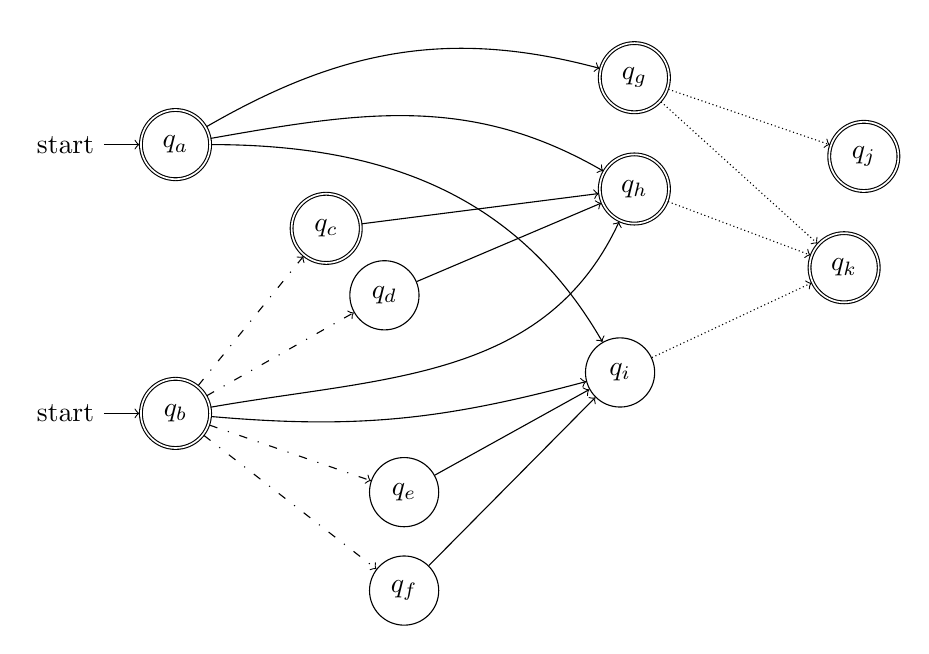
\begin{tikzpicture}[node distance=1.5cm and 3cm, auto]

\node[initial,state,accepting] (A) {$q_a$};


\node[initial,state,accepting] (B) [below= of A, yshift=-1.cm] {$q_b$};

\node[state] (F) [right= of B, yshift=-2.25cm, xshift=-1cm] {$q_f$};
\node[state] (E) [right= of B, yshift=-1.cm, xshift=-1cm] {$q_e$};
\node[state] (D) [right= of B, yshift=1.5cm, xshift=-1.25cm] {$q_d$};
\node[state] (C) [accepting, right= of B, yshift=2.35cm, xshift=-2cm] {$q_c$};

\node[state,accepting] (H)  [right= of C, yshift=0.5cm] {$q_h$};
\node[state] (I) [right= of E, yshift=1.52cm, xshift=-1.15cm] {$q_i$};

\node[state,accepting] (G) [above= of H,yshift=-1cm] {$q_g$};
\node[state,accepting] (J) [right= of G,yshift=-1cm,xshift=-1cm]  {$q_j$};

\node[state,accepting] (K) [right= of H,yshift=-1cm,xshift=-1.25cm] {$q_k$};

\path (A) edge [->, out=30, in=165, above] node {} (G)
          edge [->, out=10, in=150, above] node {} (H)
          edge [->, out=0, in=120,  above] node {} (I)
      (B) edge [->, above, loosely dashdotted]      node {} (C)
          edge [->, above, loosely dashdotted]      node {} (D)
          edge [->, below, loosely dashdotted]      node {} (E)
          edge [->, below, loosely dashdotted]      node {} (F)
          edge [->, out=10, in=245, below]  node {} (H)
          edge [->, out=-5, in=195, above] node {} (I)
      (C) edge [->, above]      node {} (H)
      (D) edge [->, above]      node {} (H)
      (E) edge [->, below]      node {} (I)
      (F) edge [->, below]      node {} (I)
      (G) edge [->, above,densely dotted]      node {} (J)
          edge [->, above,densely dotted]      node {} (K)
      (H) edge [->, above,densely dotted]      node {} (K)
      (I) edge [->, above,densely dotted]      node {} (K);
\end{tikzpicture}
\caption{Possible state transitions during a single timestamp. Accepting states are denoted with double circles. The line styles indicate the type of message: the solid line denotes a push flux from the left neighbor, the dotted line denotes a push flux from the right neighbor, the dash-dotted line denotes an update. Without loss of generality we assume that the first push flux processed arrives from the left.}
\label{fig:fsm}
\end{figure}
Our aim will be to derive a finite state machine and show that all transitions preserve the loop invariants. With 6 binary variables, we have $64$ possible states. To reduce the complexity of the system we assume that if a submesh receives a message, the first message it processes will come from the left.
All states that are attained are shown in Table~\ref{tab:firstmsg} and their transitions are pictorially shown in Figure~\ref{fig:fsm}. We note the non-standard notation depicting multiple arrows coming out of given states. These multiple arrows leaving a state are due to the fact that our binary state representation doesn't fully capture the internal state of any given submesh. In particular, when any given message is processed, the algorithm deterministically computes the appropriate transition based on the values at the cells, e.g. does the submesh need to execute an inlined update. This representation could be expanded to recover the traditional finite state machine representation at significantly greater complexity. %\Cy{this is a great explanation!}

Before we assess any state transitions,we note that the $CFL$ invariant simply checks whether or not the proposed $S_B.\tnext$ satisfies the invariant. The function {\sc compute\_t\_next}, which exclusively sets $S_B.\tnext$ is constructed to always satisfy the $CFL$ invariant, i.e. we never propose a timestep that if executed would cause a CFL violation. Thus, we will omit the invariant in the following proof. However, the proposed timesteps may be unphysically small, i.e. zero or even negative. Equation~\eqref{eq:P2} of the progress invariant will be used to ensure that all executed updates occur between intervals larger than $\Delta t_{\min}$.

We begin by noting that before any submesh has processed any event at time $\tau$, the last events must have been processed at a time strictly less than $\tau$, implying that the submesh must satisfy $b_1\land b_3 \land b_5$. In addition, since the synchronization times are only updated when two neighboring submeshes update at the same time, both $b_4$ and $b_6$ must be true. Therefore, any submesh must begin in states $q_a$ or $q_b$. These states differ based on whether or not there is an update scheduled at $\tau$.

\subsubsection{Processing Unforced Updates}
We refer to unforced updates as updates for which the \lstinline{update_forced} argument of the update function is false. All update events scheduled during the simulation are unforced updates. On the other hand, forced updates only occur as inlined events during a push flux evaluation. An unforced update will only be applied to submeshes for which $S_B.\tnext = \tau$ and $S_B.\tprev < \tau$. Otherwise, the update becomes a no-op. Thus, non-trivial update events can only be applied to submeshes in state $q_b$. %\Cy{the concept of events becoming no-ops hasn't been discussed yet, right?  Might be good to clarify the idea here.} \Max{Introduced this notion earlier when I described why there exist only a finite number of elements in a given timestep.}
\begin{enumerate}
    \item[$CR$:] Satisfying the consistency invariant before the update implies the values of the neighbors are correct until $\tau$. Therefore, the update will satisfy~\eqref{eq:CR2}. After the update, the values of the flux buffers at the edges trivially satisfy~\eqref{eq:CR3} and~\eqref{eq:CR4} since $S_B.\tprev = \tau > S_B.\ell.\tprev$. Assuming $K$ is updated appropriately in {\sc advance}, $q_b$ will satisfy the correctness invariant after the execution of an update.
    \item[$LO$:] To be locally ordered either the submesh or its neighbor must have last updated at the synchronization time. Consider the left side. If $S_B.\ell.\tprev = S_B.\ell.\tsync$, the submesh will update without causing a local ordering violation. Otherwise, the neighbor has updated since the last synchronization, and updating the submesh must be treated as a local ordering violation. In that case, $S_B.\ell.\tprev > S_B.\ell.\tsync$ and the push flux scheduled during the update will force the neighbor to update at $\tau$, meaning at some point we expect the neighbor to update at $\tau$.  Inside the submesh, the synchronization time $S_B.\ell.\tsync$ is set to $\tau$ in anticipation of the scheduled synchronization thus satisfying the local ordering invariant.
    \item[$P$:] The scheduled push fluxes satisfy~\eqref{eq:P4}.
    \item[$CI$:] Updating a submesh will cause the consistency invariant~\eqref{eq:CI1} to fail on the neighbor. However, the submesh will send a push flux. Thus, Equation~\eqref{eq:CI2} holds. If the synchronization times remain unchanged, $S_B.\ell.\tsync=S_A.r.\tsync$ continues to hold. Otherwise, the update causes a push flux, which implies that $S_B.\ell.\tsync=\tau$ and there exists a forced push flux to $S_A$.
\end{enumerate}
 Thus, $q_b$ will satisfy $I$ after processing the update. The state transition depends solely on, which sides need to receive a push flux from their neighboring submesh in order to satisfy local ordering or allow scheduling the next non-trivial update. State $q_b$ transitions to $q_c$ if no side requires updating, to $q_d$ if the left side requires updating, $q_e$ if the right side requires updating, and $q_f$ if the both sides require updating. Since the last message was received before time $\tau$, and a forced update would set $S_B.\ell.\tsync = \tau$. Precisely, $b_4$ and $b_6$ correspond to waiting on these missing flux updates. Lastly, any state that caused a forced update to be scheduled ($q_d$, $q_e$, $q_f$) cannot be terminal. The forced push flux implies that the neighbor to which that message was sent must send a push flux back if it hasn't already sent a flux. Therefore, these states will process at least one push flux.

\subsubsection{Processing the Push Flux from the Left}
Without loss of generality we assume that the first message comes from the left. Since no push fluxes have been processed, we only consider cases for which $b_3 \land b_5$ is true. Since the submesh must begin in state $q_a$ or $q_b$ and can transition to states $q_c$-$q_f$ after executing an update, it suffices to show that the invariants remain unviolated after executing the push flux on a submesh in any one of the states $q_a$-$q_f$. %\Cy{There's no context or explanation for ordering constraints.  Maybe just leave this out?}
There are three broad cases of states to consider: (i) submeshes that have not updated, but execute an inlined update during the push flux, (ii) submeshes that have not updated and do not update during the push flux, and (iii) submeshes that have already updated.
\begin{enumerate}
    \item[$CR$:] For case (i), $\tilde{S}_B.\tprev < \tau$ and the push flux causes the submesh to update. In this case, $CR$ follows by the same reasoning mentioned in the previous section. For cases (ii) and (iii), $\tilde{S}_B.\tprev = S_B.\tprev$. In the case of (iii), even if the push flux executed an inlined update, the update would be a no-op as $S_B.\tprev=\tau$. Since the push flux function doesn't modify $S_B.u$,~\eqref{eq:CR1} holds. The call to {\sc accumulate} correctly updates $S_B.\ell.\Sigma \hat{F}$ so that \eqref{eq:CR3} holds, and {\sc update\_K\_bdry} ensures that \eqref{eq:CR5} and \eqref{eq:CR6} are true. For the right side, since no modifications occur to $S_B.u$ or $S_B.r$ and the submesh is assumed to have satisfied $CR$ before the push flux, \eqref{eq:CR4}, \eqref{eq:CR7}, and \eqref{eq:CR8} must hold.
    \item[$LO$:] For case (i), the processing of the push flux and inlined update implies $S_A$ and $S_B$ are synchronized $S_B.\ell.\tprev=S_B.\tprev=S_B.\ell.\tsync$. Thus, $LO_{\ell}$ holds. On the right side, $LO_r$ will be satisfied using the same logic to ensure that $LO_r$ holds when updating a submesh. For case (ii), processing the push flux and not updating, implies that $S_A.r.\tprev=S_A.r.\tsync$. Since $S_B.\tprev < \tau$, the consistency invariant implies $S_B.\tprev = S_B.\ell.\tsync$. Therefore $LO_{\ell}$ is true. Since $S_B.\tprev$ and $S_B.r$ are unchanged $LO_r$ must hold, since it held before the push flux by assumption. Lastly, for case (iii), once the push flux has been processed at $\tau$, $LO_{\ell}$ holds by the same logic used for case (i), and since $S_B.\tprev$ and $S_B.r$ remain unchanged, $LO_r$ holds following the same logic used in case (ii).
    \item[$P$:] For case (i), the push fluxes scheduled in the inlined update satisfy \eqref{eq:P4}. For case (ii), since the message was processed and did not lead to an inlined update, $S_B.\tnext > \tau$, and an update has been scheduled satisfying \eqref{eq:P2}. For case (iii), if after the push flux we are able to schedule an update greater than $\tau$, \eqref{eq:P2} is satisfied. Otherwise, the progress guarantee and the fact that after the push flux the submesh and its left neighbor are synchronized imply that being unable to schedule a future update must arise due to the CFL condition at the right boundary, i.e. {\sc compute\_t\_next($S_B,\,S_B.r)$} $\le \tau$. When the submesh updated it must have sent a forced push flux to the right neighbor, satisfying \eqref{eq:P4}. If that push flux has already been consumed, this implies that the right neighbor has updated at $\tau$ and sent a push flux back to the submesh, satisfying \eqref{eq:P3}. Thus, \eqref{eq:P3} or \eqref{eq:P4} must hold.
    \item[$CI$:] For case (i), $S_B$ updates, and the push flux sent to $S_A$ as well as the the fact that $S_B.\ell.\tsync=\tau$ implies that~\eqref{eq:CI2} and~\eqref{eq:CI4} hold. On the right side, $CI(S_B, S_C, \tau)$ holds following the same logic used during the unforced update. For case (ii), 
    $CI(S_B,S_C,\tau)$ continues to hold since it held before the push flux was executed. Considering $CI(S_B,S_A,\tau)$, \eqref{eq:CI1} or \eqref{eq:CI2} held before the push flux. Without changes to $S_B.u_A$ or $S_B.\tprev$, one of the two statements continues to hold after the push flux. 
    Since $S_B$ did not update, $S_A$ could not have scheduled a forced update, and $S_A.r.\tsync$ remains unchanged from the state before $S_A$ last updated. Satisfying the consistency invariant on $S_B$ before any events executed at time $\tau$ implies $S_A.r.\tsync=\tilde{S}_B.\ell.\tsync$. Since the synchronization time on $S_B$ also remains unchanged \eqref{eq:CI3} must hold.
    For case (iii), $CI(S_B,S_C,\tau)$ holds following the same logic used for case (ii). On the left interface, $S_B.\ell.\tsync=\tau$ after the push flux. When $S_B$ updated at $\tau$ it sent a message to $S_A$. If this message has not been processed \eqref{eq:CI4} holds. Otherwise, $S_A$ has updated and processed the push flux for $S_B$ (in no particular order). This implies that  $S_A.r.\tsync=\tau=S_B.\ell.\tsync$. Therefore, \eqref{eq:CI3} holds.
\end{enumerate}

It is necessary to check that consuming the push flux does not lead to invariant violations of $P$ or $CI$ on $S_A$.
If $S_A$ is able to schedule a future update or still requires a message from its left neighbor (i.e. not $S_B$), consuming the push flux has no impact on $P(S_A,\tau)$. However, if $S_A$ is unable to schedule a future update due to required synchronization with $S_B$, the push flux must require an inlined update on $S_B$. If $S_B$ updates during the push flux, it will send a message to $S_A$, thereby satisfying \eqref{eq:P3}. If $S_B$ has already updated, there must be an outstanding push flux from $S_B$ to $S_A$. This event cannot have been consumed yet, since otherwise $S_A$ and $S_B$ would be synchronized on $S_A$ and the progress guarantee implies that this boundary could not hinder the scheduling of a future update. The existing push flux from $S_B$ to $S_A$ at time $\tau$ satisfies \eqref{eq:P3}. Thus $P(S_A,\tau)$ continues to hold after processing the push flux on $S_B$. 
Next, we check that $CI(S_A,S_B,\tau)$ is not violated. Since $S_A$ must have updated at $\tau$ to send the push flux and will only update once at $\tau$, we are guaranteed that $S_A$ will not have updated since sending the push flux. Therefore Equation~\eqref{eq:CI1} holds. If a push flux from $S_B$ to $S_A$ has already been processed, we know that $S_B.\ell.\tsync = \tau = S_A.r.\tsync$, satisfying \eqref{eq:CI3}. Otherwise, the outstanding push flux from $S_B$ to $S_A$ implies that~\eqref{eq:CI5} holds. Thus, processing the push flux will not violate $I$ on $S_A$.

The transitions following the execution of a push flux from the left (or right) neighbor depend on whether or not the submesh updated and whether or not it can make progress on the right side. If the submesh did not update at $\tau$---which is only the case for $q_a$---and it is able to schedule an update at a time greater than $\tau$, this will transition to $q_g$. If the mesh previously updated or is updated during the push flux, the state depends on whether or not the mesh is able to make progress on the right hand side, i.e. whether or not $b_6$ is true. 

We note that the value of $b_6$ remains unchanged for submeshes updated before the push flux. Therefore, states $q_c$ and $q_d$ will transition to $q_h$, and states $q_e$ and $q_f$ will transition to $q_i$. Submeshes which execute an inlined update transition depending on the value of $b_6$. If the submesh has issued a force push flux to its right neighbor to enforce local ordering or enable scheduling a future update, the submesh transitions to $q_i$. Otherwise, the submesh is able to make progress and the submesh transitions to $q_h$.

\subsubsection{Processing the Push Flux from the Right}
Since by assumption the first message arrives from the left, we only need to consider the right push flux applied to states after processing the push flux from the left neighbor, i.e. states $q_i$-$q_f$.
\begin{enumerate}
    \item[$CR$:] The correctness of the algorithm relies on arguments similar to those use for the push flux from the left.
    \item[$LO$:] If the push flux did not cause an update, then both sides must satisfy the local ordering constraint. Otherwise, the submesh has synchronized with both of its neighbors and satisfies the local ordering constraint on either side.
    \item[$P$:] If no update is required, that implies $S_B.\tnext>\tau$. Thus, $P$ is satisfied by \eqref{eq:P2}. Otherwise, if the submesh updated at time $\tau$, it will have already processed both neighboring push fluxes. The progress guarantee implies that the simulation will be able to schedule an update at a time greater than $\tau$, satisfying \eqref{eq:P2}.
    \item[$CI$:] The consistency invariant holds making the same arguments used to show the consistency invariant holds after processing the push flux from the left.
\end{enumerate}
In the case that push fluxes have been processed on both sides, $S_B.\ell.\tprev = S_B.r.\tprev = \tau$. Implying both $b_3$ and $b_5$ are false. In the case in which no inlined update occurred, $S_B.\tprev = S_B.\ell.\tsync < \tau = S_B.\ell.\tprev$. Otherwise, the neighbors are synchronized at time $\tau$. Therefore, $S_B.\ell.\tprev = S_B.\ell.\tsync$. Either way, $b_4$ must be true. Arguing similarly for the right side, $b_6$ must also be true. Finally, since in either case the progress guarantee was able to schedule an update for a time greater than $\tau$, $b_2$ must be true. The state transition can then be determined by whether or not the submesh updated at $\tau$, if it did not the submesh must have started in state $q_g$ and transitions to $q_j$. Otherwise, the submesh transitions to $q_k$.

\begin{remark} We note that this proof imposed no restriction on scheduling order of events with the same timestamp $\tau$. That is to say that neither update nor push flux event with the same timestamp are required to be executed before the other. However, what we have not shown here is that the events commute, i.e. given any state $q_a$ and $q_b$, any order of execution would result in the same final state along with the same messages being scheduled. Thus, while any ordering of events would provide a total variation solution, we have not shown that it would provide a unique event trace. Taking advantage of this commutativity might have performance benefits and is a topic of future work. However, for our implementation, we have enforced deterministic execution by ordering events which share a timestamp on a submesh. This is achieved by bit shifting timestamps to the left and using the extra trailing bits to break ties in timestamps.
\end{remark} %5 pages
\section{Implementation Details}
\label{sec:implementation}

By expressing the algorithm as a discrete event simulation, we can use existing parallelization infrastructure to rapidly and efficiently parallelize the proposed local timestepping algorithm. This section introduces Devastator, the parallel discrete event simulator upon which our implementation is based. Additionally, we outline several performance optimizations made to the algorithm to improve the performance as well as load balancing strategies to achieve good compute resource utilization.

\subsection{Devastator Simulation Framework}
%Need defined TimeWarp, roll back
Devastator (publication forthcoming) is the parallel discrete event simulation (PDES) framework we have used to implemented this work. As with other PDES frameworks, Devastator expects the simulation to be modeled as a discrete number of logical processes (i.e. actors) producing and consuming timestamped events. Once the logical processes and their event processing behaviors have been defined, Devastator handles the task of progressing and maintaining consistency of the distributed parallel execution. To do this, Devastator employs the TimeWarp algorithm~\cite{Jefferson1985} with an asynchronous algorithm for bounding global virtual time (GVT). Devastator was chosen for this work for its emphasis on performance in HPC environments as well as its productive C++14 interface.

PDES frameworks generally fall in one of two categories in how they maintain consistency of the distributed state, these are named optimistic and conservative. Consider the following scenario: a CPU $A$ in the simulation wants to execute event $E$ having timestamp $T$. How can the CPU be sure that no other event $E'$ with timestamp $T'$ where $T' < T$ is going to be generated by some other CPU $B$ and sent to $A$? Conservative methods require all CPUs to synchronize heavily to ensure that $E$ is only ever executed after it can be proven that no such $E'$ is possible. Optimistic methods, like TimeWarp, instead execute events optimistically before knowing that it is safe to so. To deal with the inevitable causality violations (discovering $E'$ only after executing $E$), TimeWarp performs a {\em rollback} to revert the logical process's state to before execution of $E$, then executes $E'$, then $E$, and carries on. Once GVT passes $T$, the CPU knows that no such further events $E'$ can occur, and the event $E$ is {\em committed}.

Optimistic execution enjoys the ability to operate with high performance in regimes of low communication, dynamically, simply by virtue that it always assumes no communication is needed before executing the next event. This makes it an excellent choice for domains where absolute bounds on the needed inter-CPU synchronization are far tighter than what is required in the average case. Simply put, for an application that rarely needs to communicate, it's best to assume it never needs to and then only pay a heavy cost when that assumption fails, rather than synchronizing frequently (as in a conservative execution) only to learn communication isn't required.

 In the case of nonlinear conservation laws, determining whether an event is able to execute without incurring a CFL violation requires determining the domain of dependence for that submesh. Due to pathological examples such as the shockwave for Burgers' equation considered in the introduction, this is an inherently non-local problem. In situ computation of the domain of dependence would greatly increase required communication between submeshes. The locality of this problem can be limited by considering smaller timesteps at the cost of available parallelism. However, in practice we assume that the probability of a remote high-speed wave dramatically increasing $|\Lambda|$ and causing CFL violations is very small. Using optimistic execution, we are able to maintain our local communication stencil without limiting parallelism, and only incur significant overhead when timesteps require refining.

\subsection{Performance related optimizations}
While implementing the above presented push flux and update functions specify a TVD timestepping algorithm, three performance optimizations were necessary to obtain good parallel performance.
\begin{enumerate}
    \item {\em Timestep binning:} While the {\sc compute\_t\_next} allows us to take optimally large timesteps, the local ordering constraint makes this approach suboptimal. As an example consider two neighboring submeshes, which are able to take respective timesteps of 16 (the left submesh) and 17 (the right submesh) time units. During the simulation, the left submesh advances to time 16, and the right submesh advances to time 17. Once the right submesh has advanced, it forces its neighbor to update due to a local ordering violation, and so the left submesh has updated at both times 16 and 17. Using a work-depth analysis, at time 272, this approach requires $3\cdot 16$ (48) updates, and has a depth of $2\cdot 16$ (32). Instead, we propose binning timesteps to the nearest power of two. Specifically, we require that given a certain timestep size ($\Delta t$), we step to largest multiple of the largest power of two multiplied by $\Delta t_{\min}$ less than the given timestep. This naturally synchronizes submeshes and avoids extra updates due to local ordering violations. In the given example, both submeshes would take timesteps of 16. Thus, the work would be $17\cdot 2$ (34) and the depth would be 17. By restricting allowable timestep sizes, we potentially reduce both work and the depth of the simulation.
    \item {\em Reducing unnecessary speculation:} While TimeWarp allows us to speculatively update the submeshes, it is not always wise to do so. If a submesh updates and sends a forced push flux to one neighbor, we know that at that time the neighbor would have to send a push flux back. Therefore, any events executed on the submesh before the neighboring push flux arrives must be rolled back. Therefore, whenever scheduling new updates the submesh inspects its state to determine whether it is still waiting for a message from one of its neighbors. If so, it will simply return without scheduling any further events. Once the messages the submesh is waiting on arrive, it will schedule the next events without having to roll back events.
    \item {\em Avoiding small timesteps due to binning:} While timestep binning reduces the number of synchronizations required due to local ordering violations, it introduces another problem due to the fact that timesteps at submesh boundaries are computed relative to the previous synchronization time. Considering two submeshes that both could step at 7 time units. The timestep binning would make both of these submeshes update at time 4. However, assuming that the push flux from one submesh is delayed, the other submesh would take timesteps of sizes 2 and 1 before being unable to make progress and sending a forced update to the neighbor. Since the timestep is taken relative to the previous synchronization time, the submesh will try to enumerate the bits of its maximum timestep before waiting on a message from its neighbor. This phenomena is highly problematic for parallel discrete event simulation, since once the neighboring message at time 4 arrives, the updates at times 6 (timestep of 2) and 7 (timestep of 1) would have to be rolled back along with any events scheduled due to those later updates. Furthermore, since the timesteps become smaller and smaller, the associated updates are enqueued with a high priority into the event queue and the simulator is more likely to spend time executing events which will be rolled back.  To remedy this, we introduce a heuristic whereby we examine the ratio between the timestep taken if the submesh were synchronized with its neighbors divided by the computed timestep due to a single neighbor, i.e. the value of {\sc compute\_t\_next\_bdry}. If this ratio is greater than or equal to 2, we force that neighbor to update at the current time. The previous optimization (reducing unnecessary speculation) then causes the submesh to wait until the neighbor's push flux has been processed. While this may increase the critical path of simulation depending on the latency associated with sending messages, we have found that in practice this significantly reduces bad speculation.
\end{enumerate}

\subsection{Performance Modeling and Load Balancing}
\label{sec:load-balancing}
To understand the performance results as well as load balance the problem, we estimate the work for a given problem as follows. At a given simulation time $\tau$, the timestep $dt$ taken by cell $j$ can be approximated as
\begin{equation*}
dt_j(\tau) = \Delta t_{\min} 2^{\left\lfloor \log_2 \frac{ \Delta x_j}{2 |\Lambda(\tau, x_j)| \Delta t_{\min}}\right\rfloor},
\end{equation*}
where $\Delta t_{\min}$ is the smallest timestep, $\Delta x_j$ is the cell size, and $|\Lambda|$ corresponds to the wave speed at time $\tau$ in the midpoint of the cell. The $\log_2$  appropriately bins the timesteps.

The mesh partitioning problem follows a 2-phase process of aggregating cells into submeshes and assigning the submeshes to ranks. Cells within each submesh step synchronously enabling efficient utilization of CPU architectures. Although stability requirements necessitate that cells step at the most stringent timestep of cells associated with that submesh, unstructured finite element meshes typically exhibit small variations of timestep sizes in a given neighborhood. Therefore, the synchronous stepping inside a submesh marginally decreases the maximum attainable speed-up.

The mapping of cells to submeshes is denoted by $\pi:\mathbb{Z} \to \mathbb{Z}$.
Since in this chapter, we exclusively consider one dimensional problems, we define our partition using a set of ordered splitters $\{s_i\}\subset \mathbb{Z}$ where the submesh $i$ has been assigned the cells with indices $[s_i,s_{i+1})$. The relationship between the splitters and partition function is then given by: for cell $j$, $\pi(j) = i^*$ such that $s_{i^*} \le j < s_{i^*+1}$. %\Cy{also, keep capitalization of $s_i$ vs. $S_i$ consistent}
%\Cy{consider using $j$ as the index for meshes and $i$ as the index for cells}\Max{$j$ is for cells and $i$ is for submeshes. This is consistent with earlier parts of the paper too}
For the generation of $\pi$, we assume no prior knowledge on $\Lambda$ i.e. $|\Lambda| \equiv 1$, and partition solely based on variation in cell sizes. 
Let $w_j$ be the weights assigned to each cell. Each $w_j$ is determined by the smallest allowable timestep on a given submesh, i.e.
\begin{equation*}
w_j = \frac{1}{\min_{1\le r \le n_{el}}\{dt_r(\tau) \, : \, \pi(j) = \pi(r) \}}.
\end{equation*}
Since the partitioner balances work across submeshes, but the work depends on the partitioning, there exists a circular dependency.
Hence, we generate $\pi$ using an iterative procedure. Given weights $\{w_j\}$, we create a partition $\pi$, ensuring each submesh has the same amount of work.
 With the new partition, update the weights $w_j$, which may change based on elements added or removed from a submesh. Repeat this process until some terminating condition is satisfied. In this thesis, we stop iterating after 100 iterations. Throughout the iterations, we track the amount of work assigned to the most overworked submesh. At the end of the iterative procedure, we return the partition with the least overworked submesh, i.e. if $\pi_{\ell}$ is the $\ell$-th iteration of the submesh partitioner, 
\begin{equation*}
\pi = \argmin_{\{\pi_{\ell}\}} \max_{0 < i < \nsbmsh} \sum_{j=1}^{n_{el}} \chi_{\{\pi_{\ell}(j) = i\}}(j) w_{j}
\end{equation*}
where $\chi_A$ denotes an indicator function over set $A$. The objective of the first partitioning phase is to specify a problem that can be efficiently executed by the parallel discrete event simulator. The proposed scheme attempts to generate submeshes such that the number of cells updated is approximately equal across all submeshes. However, due to the dependence of work on partitioning, we must also pay attention to the total work. A proposed partitioning may be perfectly load balanced but require a lot more work and therefore be less preferable than a partitioning which is imbalanced but more work optimal, i.e. for which the discrepancy between $w_j$ and $dt_j^{-1}$ is smaller.

%\Cy{whereas the objective of the first phase was to equalize estimated work across submeshes, without using/requiring wavespeed?} 
The second partitioning phase assigns submeshes to ranks. The objective of this phase is to minimize the runtime of the simulation. Let $\rho$ map a submesh to its assigned rank. Since the most overworked rank will determine the rate at which global virtual time is advanced, we estimate the wall-clock time as
\begin{equation}
T = \int_0^{\tend} \max_{0 \le k < n_{ranks}} \sum_{j=1}^{n_{el}}  w_j(\tau) \chi_{\{(\rho \circ \pi)(j) = k\}}(j) \,\mathrm{d} \tau.
\label{eq:lb}
\end{equation}
%\Cy{consider replacing $(\rho \circ \pi)^{-1}(k)$ with $(\rho \circ \pi)(i) = k$ or maybe $i \in (\rho \circ \pi)^{-1}(k)$}
%\Cy{looks like the definition of $w$ has changed since the previous definition to take into account wave speed?}
We remark that for performance results presented in Section~\ref{sec:performance-results}, we consider analytic solutions, thereby yielding a good approximation to $|\Lambda|$ and hence $w_j$. We solve \eqref{eq:lb} using a Gauss-Lobatto quadrature to approximate the integral in time. Given the submesh partition $\pi$ and our assumed wavespeed $\Lambda$, we can formulate this problem as mixed integer programming problem, which we solve using Gurobi~\cite{Gurobi}.  The incorporation of $|\Lambda|$ in \eqref{eq:lb} introduces a discrepancy between the $|\Lambda|$ used for the two partitioning phases. The decision to use different $|\Lambda|$ for the partitioning phases arises from two considerations. First, exactly knowing $|\Lambda|$ is an impractical constraint. Since $|\Lambda|$ is a function of the solution, knowing $|\Lambda|$ implies already knowing the solution to the problem we are interested in solving. Using approximations or even analytic representations of $|\Lambda|$ for determining $\pi$ can be problematic. If we consider one giant submesh and a single cell underestimates $|\Lambda|$, the entire submesh will incur extra work. By ignoring $|\Lambda|$ in during the computation of $\pi$, we inoculate ourselves against adverse effects caused by poor estimates of $|\Lambda|$. The second consideration has to do with partitioner performance. The number of cells is 2-3 orders of magnitude larger than the number of submeshes. Attempting to solve \eqref{eq:lb} for the cell graph would be intractable for large cell counts. By ignoring $|\Lambda|$ in the first partitioning phase, we can use existing fast graph partitioners to generate submeshes and use more sophisticated means to achieve good load balance at the submesh level.

Lastly, we derive upper limits on the speed-up achievable as the ratio of work (i.e. number of cell updates) executed by a standard synchronous timestepping implementation using an MPI runtime divided by the local timestepping Devastator implementation. We calculate the total work for the Devastator runtime as
\begin{equation*}
W^{th}_{deva} = \sum_{j=1}^{n_{el}} \int_0^{\tend} w_{j}(\tau) \, \mathrm{d} \tau.
\end{equation*}
Note that this estimate is a conservative work estimate for the Devastator implementation as it doesn't account for factors such as taking intermediate timesteps between finer and coarser timesteps as well as extra timesteps due to forced updates and rollbacks. For an MPI-based implementation, which steps with uniform timesteps, we compute the work $W^{th}_{MPI}$ as the number of timesteps times the number of elements.
We bound the largest theoretical speed-up by
\begin{equation*}
    S^{th} = \frac{ W^{th}_{MPI}}{W^{th}_{deva}}.
    %\label{eq:Sth}
\end{equation*}
This will provide a baseline to assess how efficient the implementation is.

\subsection{Ease of Implementation}

\begin{figure}
    \centering
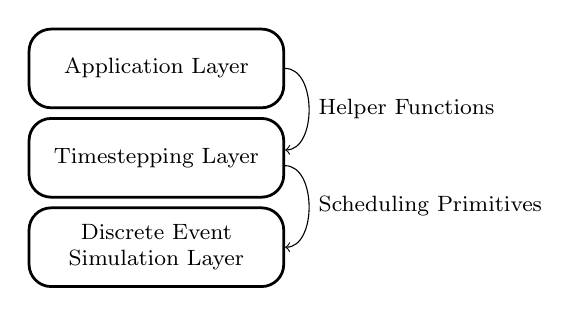
\begin{tikzpicture}[->,node distance=0.1cm,
rnd/.style={
  draw=#1,
  rounded corners=8pt,
  line width=1pt,
  align=center,
  text width=3cm,
  minimum height=1cm,
  font=\footnotesize
  }
]
\node[rnd] (AL) {Application Layer};
\node[rnd, below=of AL] (TL) {Timestepping Layer};
\node[rnd, below=of TL] (DL) {Discrete Event Simulation Layer};

\path (AL.east) edge [bend left=90] node[right] {\footnotesize Helper Functions} ([yshift=1mm] TL.east)
      ([yshift=-1mm] TL.east) edge [bend left=90] node[right] { \footnotesize Scheduling Primitives} (DL.east);
\end{tikzpicture}
\caption{Stack Diagram for the Local Timestepping Implementation}
\label{fig:stack-diagram}
\end{figure}

We conclude this section by remarking on the complexity of the implementation. The proposed algorithm can be segmented into three main software layers shown in Figure~\ref{fig:stack-diagram}. At the lowest level is the discrete event simulation layer for which we are using Devastator. Devastator handles all parallelism via the scheduling primitives (Definition~\ref{def:scheduling-primitives}). The layers on top of it schedule events and Devastator ensures that the events are executed in the correct order in a parallel setting. On top of the Devastator layer is the timestepping layer. This layer contains the timestepping logic introduced in Section~\ref{sec:alg}. The complexity of running in an asynchronous context makes this layer difficult to reason about without a tool like loop invariants. However, through judicious specification of helper functions (Definition~\ref{def:helper-functions}) we can prevent the complexity of the timestepping algorithm from seeping into the topmost layer, the application layer. In practice, the timestepping algorithm should be wrapped into a library, and the user would solely need to implement the helper functions. At this highest level, features of the algorithm such as numerical discretization and the form of the conservation laws are specified. Programming at this highest level is effectively identical to programming flat MPI code. The {\sc advance} function is essentially the main kernel of an MPI rank. The only additional calls that need to be supplied deal with assessing the appropriate timestepping size and what to do once a submesh update is either committed or rolled back. This segmentation facilitates the introduction of local timestepping into existing scientific applications without requiring extensive rewriting of code or impeding productive software development in the application layer.

\section{Results}
\label{sec:results}
\begin{figure}
  \centering
  \subfloat[Uniform]{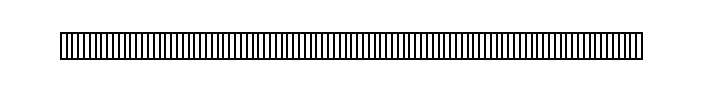
\includegraphics{adaptive_local_timestepping/images/mesh_uniform}}\\
  \subfloat[Polynomial]{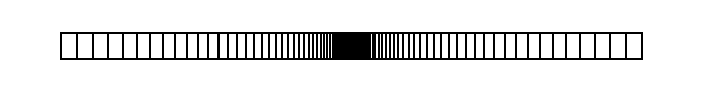
\includegraphics{adaptive_local_timestepping/images/mesh_polynomial}}\\
  \subfloat[Piecewise]{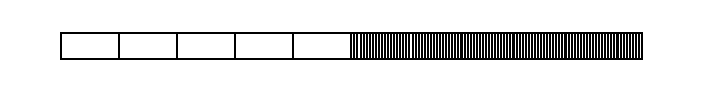
\includegraphics{adaptive_local_timestepping/images/mesh_piecewise}}
  \caption{Meshes used for numerical experiments}
  \label{fig:meshes}
\end{figure}

In this section we present results for the one dimensional Burgers' equation and the shallow water equations. Since the timestepping method is first order, we only consider first order finite volume schemes.
To demonstrate the robustness of the timestepping method for different types of meshes, we consider three meshes: a uniform mesh, a polynomial mesh, and a piecewise mesh. These meshes are generated by warping uniformly distributed nodes along $(-1,1)$ onto the interval $(-1,1)$. The base case is the uniform mesh for which the warp function is the identity, i.e. $w(x) = x$. The polynomial mesh refines the mesh around the origin. This type of mesh is common for finite element applications where local refinement is required to resolve flow around fine features. The warp function for this mesh is given as
\begin{equation*}
  w(x) = \frac{1}{1/3 + \varepsilon} \left( \frac{ x^3}{3} + \varepsilon x \right),
\end{equation*}
where we set $\varepsilon = 0.02$ in order the bound the ratio of largest to smallest cells. Lastly, we consider a mesh with a large jump in refinement. The warp function is then defined so that the ratios of cell sizes is at least 16 to 1. Assuming the nodes are enumerated $x_{j}$ for $0 \le j \le n_{el}$, define $j^*  = \lfloor n_{nodes}/17 \rfloor$. We then define the warp function for the piecewise mesh as
\begin{equation*}
  w(x) = \begin{cases}
    \frac{x + 1}{1 + x_{j^*}} - 1 & \text{for } j \le j^*\\
    \frac{x - 1}{1 - x_{j^*}} + 1 & \text{for } j > j^*\\
    \end{cases}.
\end{equation*}
For clarity the meshes used are depicted in Figure~\ref{fig:meshes}. To illustrate the behavior of the timestepping algorithm, we consider meshes with 100 cells and 20 submeshes in the next two sections.  In practice, the number of cells per submesh needs to be significantly larger to amortize runtime overheads with useful work. Section~\ref{sec:performance-results} showcases performance results with meshes consisting of 500,000 cells.

%additional performance considerations
%CFL condition


\subsection{Burgers' Equation}
Consider Burgers' equation on the line,
\begin{equation}
\partial_t u + \partial_x u^2/2 = 0.
\end{equation}
We consider two sets of initial conditions: firstly, the shockwave, which is initialized
\begin{equation*}
  u_0(x) = \begin{cases}
    1 & x < 0\\
    0 & x > 0,
    \end{cases}
\end{equation*}
and secondly a rarefaction wave,
\begin{equation*}
  u_0(x) = \begin{cases}
    -1 & x < 0\\
    1 & x > 0.
  \end{cases}
\end{equation*}

\begin{figure}
  \centering
  \subfloat[Uniform-Shockwave\label{fig:burgers:spacetime:uniform:shockwave}]{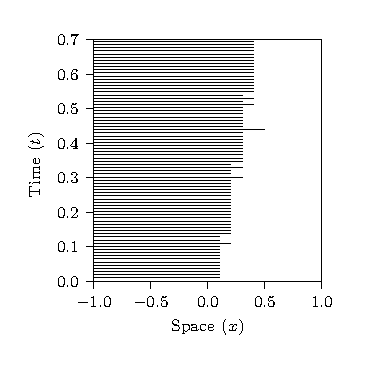
\includegraphics{{adaptive_local_timestepping/images/event_trace_burgers_uniform_shockwave}}}
  \hfill
  \subfloat[Uniform-Rarefaction\label{fig:burgers:spacetime:uniform:rarefaction}]{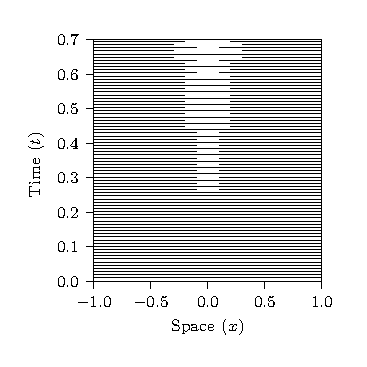
\includegraphics{{adaptive_local_timestepping/images/event_trace_burgers_uniform_rarefaction}}}
  \\
  \subfloat[Polynomial-Shockwave\label{fig:burgers:spacetime:polynomial:shockwave}]{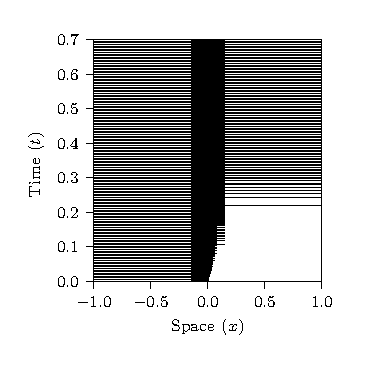
\includegraphics{{adaptive_local_timestepping/images/event_trace_burgers_polynomial_shockwave}}}
  \hfill
  \subfloat[Polynomial-Rarefaction\label{fig:burgers:spacetime:polynomial:rarefaction}]{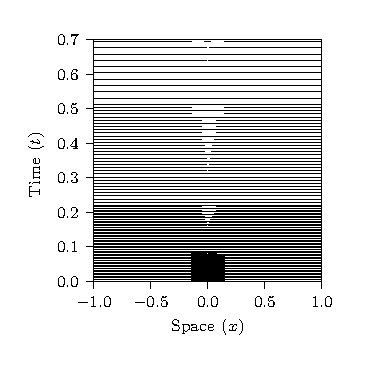
\includegraphics{{adaptive_local_timestepping/images/event_trace_burgers_polynomial_rarefaction}}}
  \\
  \subfloat[Piecewise-Shockwave\label{fig:burgers:spacetime:piecewise:shockwave}]{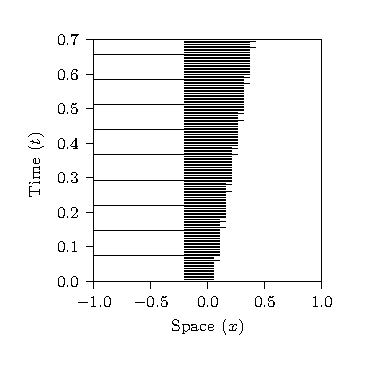
\includegraphics{{adaptive_local_timestepping/images/event_trace_burgers_piecewise_shockwave}}}
  \hfill
  \subfloat[Piecewise-Rarefaction\label{fig:burgers:spacetime:piecewise:rarefaction}]{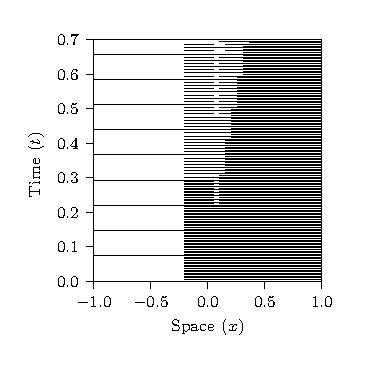
\includegraphics{{adaptive_local_timestepping/images/event_trace_burgers_piecewise_rarefaction}}}
  \caption{Space-time plots for Burgers' equation with various meshes and problem configurations.}
  \label{fig:burgers:spacetime}
\end{figure}


For both cases, we enforce the boundary conditions by setting the boundary value to the analytic solution. We note that these test cases highlight the ability of the local timestepping algorithm to refine the timestep---in the case of the shockwave---and the ability to coarsen the timestep---in the case of the rarefaction. To visualize the timesteps taken by these algorithms, we present space-time event traces similar to those shown in Fig.~\ref{fig:sol-cartoon}. In these plots, the $x$-axis corresponds to the domain $\Omega$, and the $y$-axis represents simulation time, each line corresponds to an update having executed at that given time. The space-time plots are shown in Fig.~\ref{fig:burgers:spacetime}.  For the shockwave and rarefaction problems on the uniform polynomial mesh, the $L^1$- and $L^2$-errors are bounded by 0.055. For the piecewise mesh, the errors are bounded by 0.15. Nevertheless, results for the piecewise mesh remain stable and show that the under resolved region is able to step with much larger timesteps. Looking at Figures~\ref{fig:burgers:spacetime:uniform:shockwave} and \ref{fig:burgers:spacetime:piecewise:shockwave}, we see that submeshes only update behind the shock front. For the shockwave initial conditions on the polynomial mesh---shown in Figure~\ref{fig:burgers:spacetime:polynomial:shockwave}---after $t=0.2$ the entire mesh begins stepping. This is due to the fact that cells in the interval $(0.146, 1)$ belong to a single submesh. Since these cells take larger timesteps the submesh partitioner places more cells into this submesh. In later results with more cells and submeshes, the inactive regions of the polynomial mesh do not update.
For the rarefaction problem, due to timestep binning, timestep coarsening happens only once the submesh is able to take a timestep twice as large as the previous timestep. 
For the analytic solution to the rarefaction wave at $t=0.7$--the end of the simulation---$|u|<0.5$ for $|x|<0.35$. This is consistent with the observed timestep  coarsening seen in Figure~\ref{fig:burgers:spacetime:uniform:rarefaction}. Similarly, the polynomial and piecewise meshes are able to adapt their timesteps appropriately. In these cases, the submesh partitions are not symmetric about $x=0$, giving rise to the asymmetry in the event traces.
 %\Cy{Consider adding a little more discussion about the Figures.  What should the reader be looking for and learning from them as you compare across mesh geometry and boundary conditions?}


\subsection{Shallow Water Equations}
In order to show that the local timestepping scheme is robust for more non-linear problems and in the absence of the theoretical guarantees, we provide two problems for the shallow water equations. Consider the system of conservation laws,
\begin{equation*}
  \begin{cases}
    \partial_t h + \partial_x q_x = 0 &\\
    \partial_t q_x + \partial_x ( hu^2 + gh^2/2) = -gh\partial_x z&\\
  \end{cases}
\end{equation*}
where $q_x = hu$, $z$ is the bathymetry, and $g=1$. We consider here the dam break Riemann problem, for which,
\begin{align*}
  h_0(x) &= \begin{cases}
    1 & \text{if } x < 0,\\
    1/16.1 & \text{if } x > 0,
  \end{cases}\\
  q_{x,0}(x) &= 0,\\
  z &= 0.
\end{align*}
For the shallow water equations the maximum advection speed, $|\Lambda|$ is  $\sqrt{gh} + |u|$. The initial conditions have been chosen to allow a 4-to-1 timestepping ratio between downstream and upstream of the dam break for the uniform mesh. The second shallow water test case we consider is the analytic problem of Carrier and Greenspan~\cite{Carrier1958}. This problem considers water moving up and down a shoreline with uniform slope in a periodic manner. We follow the set-up outlined in~\cite{Bokhove2005} with a phase shift of $\varphi=-\pi$.

For the numerical discretization, we use a local Lax-Friedrichs flux along with the first-order local hydrostatic reconstruction proposed in~\cite{Audusse2004}. The space time plots are shown in Figure~\ref{fig:swe:spacetime}.  We note that for the shallow water flow, the theoretical guarantees no longer hold. In fact, the timestepping region between the two waves emanating from the dam break problem in Figure~\ref{fig:swe:spacetime:uniform:dambreak} requires a finer timestep than observed during the beginning of the simulation, and thereby violates the progress guarantee, Lemma~\ref{lem:progress-guarantee}. For the dam break problem, the refinement of the timesteps looks similar to that of the shockwave problem for Burgers' equation. For the uniform and piecewise meshes, we see expected refining of timestep sizes, and for the polynomial mesh, regions far from the shock waves prematurely begin taking fine timesteps due to the large submeshes generated by the submesh partitioner.

For the Carrier-Greenspan problem on the uniform mesh, shown in Figure~\ref{fig:swe:spacetime:uniform:cg}, we see the wave moving in and out of the domain. Analytically, the water front never goes past $x=0.25$, and the simulated event trace reflects this as no submesh updates occur for in regions for which $x>0.3$.  For the polynomial mesh in Figure~\ref{fig:swe:spacetime:polynomial:cg}, we again begin stepping everywhere due to the submesh graph partitioning. For both of these cases, we note hysteretic effects in regions which are mesh drying. The final simulation time of $2 \pi$ contains two periods of the Carrier-Greenspan solution. At time $\pi$,  the submeshes participating in updates would ideally look identical to the start of the simulation, i.e. only submeshes which contain cells located at $x<-0.25$ would update. Rather we see this slow ``draining'' of mass as submeshes try to coarsen their timesteps, resulting in updates occurring in regions of the mesh that are dry in the analytic solution. The impact of behavior on performance will be touched upon in the next section. For the piecewise mesh, the incoming wave is so under resolved that it is unable to cause significant wetting and drying on the beach. Hence, this configuration fails to reproduce the periodic wetting and drying event trace seen for the uniform and polynomial meshes.

To conclude, the proposed timestepping method remains stable for simulations with dramatic temporal variations in $\Lambda$ as shown for Burgers' equation in Figure~\ref{fig:burgers:spacetime} and the shallow water equations in Figure~\ref{fig:swe:spacetime}. For the latter problem, we fail to satisfy the assumptions for the proof of correctness and even observe a violation of the progress guarantee, and yet the algorithm is able to stably compute the correct solution. Important in both problems is the ability for the algorithm to locally refine or coarsen timesteps. The proposed formulation dispenses with complicated book keeping relating to which timestepping level submeshes are in and how to appropriately define buffer zones, but simply computes and adjusts the timestep based on locally available information.


%\Cy{Again, a little more discussion would be nice.  Maybe point out advantages and disadvantages of the different mesh geometries for the different problems?}
\begin{figure}
  \centering
  \subfloat[Uniform-Dam break\label{fig:swe:spacetime:uniform:dambreak}]{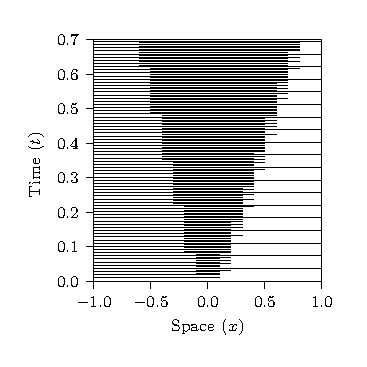
\includegraphics{{adaptive_local_timestepping/images/event_trace_swe_uniform_dambreak}}}
  \hfill
  \subfloat[Uniform-Carrier-Greenspan\label{fig:swe:spacetime:uniform:cg}]{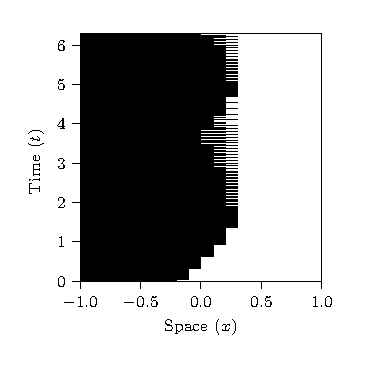
\includegraphics{{adaptive_local_timestepping/images/event_trace_swe_uniform_carrier-greenspan}}}
  \\
  \subfloat[Polynomial-Dam break\label{fig:swe:spacetime:polynomial:dambreak}]{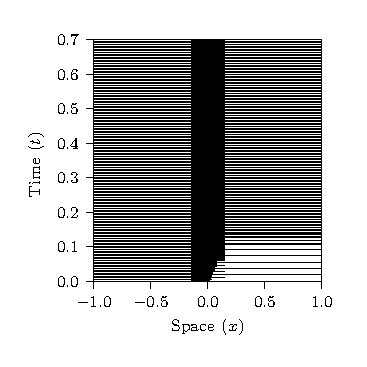
\includegraphics{{adaptive_local_timestepping/images/event_trace_swe_polynomial_dambreak}}}
  \hfill
  \subfloat[Polynomial-Carrier-Greenspan\label{fig:swe:spacetime:polynomial:cg}]{\includegraphics{{adaptive_local_timestepping/images/event_trace_swe_polynomial_carrier-greenspan}}}
  \\
  \subfloat[Piecewise-Dam break\label{fig:swe:spacetime:piecewise:dambreak}]{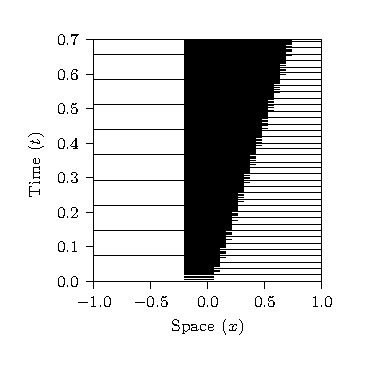
\includegraphics{{adaptive_local_timestepping/images/event_trace_swe_piecewise_dambreak}}}
  \hfill
  \subfloat[Piecewise-Carrier-Greenspan\label{fig:swe:spacetime:piecewise:cg}]{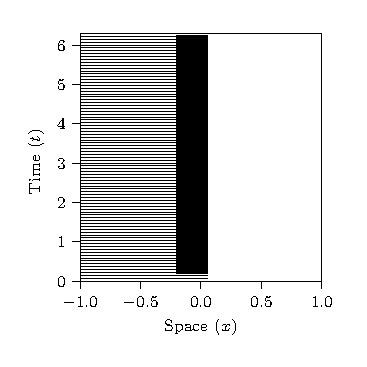
\includegraphics{{adaptive_local_timestepping/images/event_trace_swe_piecewise_carrier-greenspan}}}
  \caption{Space-time plots for the shallow water equations with various meshes and problem configurations.}
  \label{fig:swe:spacetime}
\end{figure}

\subsection{Performance Comparison}
\label{sec:performance-results}

In this section, we compare the performance of our local timestepping implementation to a flat MPI implementation. For the MPI implementation, we use non-blocking point to point messaging and hide message latencies with internal work. For more details, we refer the reader to implementation in~\cite{Bremer2019}. One key detail is that the MPI implementation does not compute the CFL condition, but rather uses a fixed timestep. Since dynamically updating a CFL condition would require an all-reduce at each timestep, the communication overhead makes an adaptive CFL condition non-viable for large-scale simulation. For the performance comparison, we consider the uniform and polynomial mesh with 500,000 cells on one Skylake node with 48 cores on TACC's Stampede2. A detailed overview of the computing environment as well as simulation parameters are presented in Appendix~\ref{sec:artifact}. We partition the mesh into 48 (one per core) uniform submeshes for the MPI implementation, and 288 (six per core) submeshes for the Devastator implementation based on the heuristic described in Section~\ref{sec:load-balancing}. %\Cy{may want to mention the reason for over-decomposition}
The over-decomposition factors of submeshes to ranks have been optimized for each runtime.
Over-decomposition of the mesh for Devastator enables three performance optimizations.
Firstly, over-decomposition allows a rank to hide message latencies. While one actor may be waiting on a message to arrive, the rank may execute events scheduled for other actors. 
Secondly, over-decomposition reduces the total amount of work required. Since each cell must step synchronously with other cells on that submesh, creating more submeshes implies that more cells are able to step with different timesteps. 
Lastly, more submeshes improves the performance of the load balancer. With more submeshes, the load balancing algorithm is able to more easily balance the simulation throughout all time points in the simulation. However, over-decomposition  comes at the cost of higher runtime overhead. More events with less work implies that a larger fraction of event execution time is spent on scheduling and control flow. The over-decomposition factor of 6 was chosen based on observed performance.
The MPI implementation does not benefit from over-decomposition. We explicitly hide message latencies by performing all internal work after posting sends and receives. Furthermore, the total number of cell updates---and thus work---remains independent of the over-decomposition factor and the load balancer is able to balance work across MPI ranks easily. 

To analyze the impact of the dynamic CFL condition versus the local timestepping due to mesh refinement, we consider two problems for the shallow water equations. Firstly, we consider a lake at rest problem, where
\begin{align*}
h_0(x) &= 1,\\
q_{x,0}(x) &= 0,\\
z &= 0.
\end{align*}
For this problem, differences in the CFL condition are solely a function of differences in cell size, $\Delta x$. The second problem we consider is the Carrier-Greenspan solution, outlined in the previous section. As the water front moves across the mesh, large portions of the mesh wet and dry throughout the simulation, causing these regions to experience large changes in allowable timestep sizes. For the lake at rest problem, the work in each submesh is approximately the same. Thus, we assign submeshes $[6\cdot k, 6 \cdot(k+1))$ to rank $k$. In the case of the Carrier-Greenspan problem, due to the periodic nature of $|\Lambda|$, we load balance over a quarter of the period, i.e. $\tend=\pi/2$ in~\eqref{eq:lb}. The performance data is shown in Table~\ref{tab:performance-data}. For the static uniform Lake at Rest problem, we include a Devastator configuration---labeled as (no CFL)---without the overhead of computing the local CFL in order to provide a more direct comparison with the MPI version, which does not compute the CFL in any configuration.  Each configuration is run 10 times with the average time elapsed, $\bar{T}$ reported in seconds. The standard deviation over the mean $\sigma_T/\bar{T}$ is given in percentages. Lastly, the number of updates and rollbacks are taken from a single run.  

We begin by noting that the number of cells rolled back is limited. At most 3.5\% of updates are rolled back suggesting that the performance related optimizations do a good job of preventing unnecessary rollback. The lack of rolled back updates for the uniform mesh lake at rest problem shows that we are able to completely avoid bad speculation for this configuration. For the lake at rest problem on the polynomial mesh, it should be possible to infer when messages are incoming since $|\Lambda|$ and $\Delta x$ are fixed. The existence of rollbacks implies that there is still future work to be done to prevent bad speculation.

\begin{table}
{\footnotesize
\caption{Execution times for the shallow water equations on Stampede2.}
\label{tab:performance-data}
  \centering
%This file is generated as part of a script. Instead of directly editing it
%please make the appropriate changes in images/src/raw_performance_data.py

\begin{tabular}{|c|c|c|c|c|c|c|c|c|} \hline
Problem & Mesh & Runtime & $\bar{T}$ & $\sigma_T/\bar{T}$ & $\#$ of Updates & $\#$ of Rollbacks\\\hline
Lake at Rest & Uniform & Devastator (no CFL) &  139.4 & 0.8\% & $252.5\cdot 10^9$ & 0 \\\hline
Lake at Rest & Uniform & Devastator &  173.2 & 0.8\% & $252.5\cdot 10^9$ & 0 \\\hline
Lake at Rest & Uniform & MPI &  133.2 & 0.1\% & $252.5\cdot 10^9$ & -- \\\hline
Lake at Rest & Polynomial & Devastator &  192.6 & 3.3\% & $239.7\cdot 10^9$ & $  3.5\cdot 10^9$ \\\hline
Lake at Rest & Polynomial & MPI &  478.4 & 2.0\% & $892.2\cdot 10^9$ & -- \\\hline
Carrier-Greenspan & Uniform & Devastator &  729.4 & 1.1\% & $856.2\cdot 10^9$ & $ 12.0\cdot 10^9$ \\\hline
Carrier-Greenspan & Uniform & MPI &  995.7 & 0.7\% & $1674.5\cdot 10^9$ & -- \\\hline
Carrier-Greenspan & Polynomial & Devastator & 3212.4 & 0.5\% & $3209.6\cdot 10^9$ & $113.3\cdot 10^9$ \\\hline
Carrier-Greenspan & Polynomial & MPI & 10732.0 & 0.1\% & $18070.1\cdot 10^9$ & -- \\\hline
\end{tabular}
}
\end{table}


\begin{table}
{\footnotesize
\caption{Theoretical versus observed speed-ups.}
\label{tab:speed-ups}
  \centering
\include{adaptive_local_timestepping/images/speedups}
}
\end{table}
The speed-up achieved via local timestepping is attained through work reduction. 
To assess the quality of our implementation, we contextualize execution times with configuration-dependent metrics to determine what fraction of unnecessary work was skipped. 
Recall the theoretical speed-up $S^{th}$, which estimates the maximum achievable speed-up based on analytic values of $\Lambda$ and $\Delta x$. We compare this theoretical estimate against a speed-up based on the number of cells updated.
 Let $W^{obs}_{MPI}$ and $W^{obs}_{deva}$ be the number of cells updated during the simulation with respective runtimes, and define the work-based speed-up as $S^{work}$ the ratio of observed updates, i.e.
\begin{equation*}
S^{work} = \frac{W^{obs}_{MPI}}{W^{obs}_{deva}}.
\end{equation*}
Discrepancies in $S^{work}$ and $S^{th}$ arise due to the enforcing of the local ordering constraint as well as extra updates arising from a combination of timestep binning and variations in $\Lambda$.

Lastly, we introduce the observed speed-up, which is based on the ratio of run times,
\begin{equation*}
S^{obs} = \frac{ \bar{T}_{MPI} }{\bar{T}_{deva}},
\end{equation*} 
where $\bar{T}_*$ corresponds to the mean observed execution time for either runtime. While the work based speed-up $S^{work}$ represents an upper bound on achievable speed-up, the observed speed-up is able to take into consideration factors such as imbalance, rollbacks, and algorithmic overhead.

Table \ref{tab:speed-ups} presents the three speed-up values for each configuration. The discrepancies between $S^{th}$ and $S^{work}$ are less than 3\% with the exception of the Carrier-Greenspan polynomial configuration where we over-predict the attainable speed-up by 17\%. In particular, we suspect these discrepancies result due to difficulties in water draining out of dry regions akin to the updates seen in Figures~\ref{fig:swe:spacetime:uniform:cg} and \ref{fig:swe:spacetime:polynomial:cg}.

 The observed speed-up ranges from $\minSObsOverWork\%$ to $\maxSObsOverWork\%$ of the work-based theoretical speed-up, $S^{work}$. 
 Since there is no theoretical benefit from using adaptive, local timestepping in the lake at rest on a uniform mesh configuration, this case highlights the overhead associated with using an adaptive, local timestepping scheme versus a static synchronous timestepping scheme. If we skip the CFL computation and use the analytic value of $K^{\intr}$ (see the first row of Table~\ref{tab:performance-data}), the observed speed-up is  $S^{obs}=\SobsNoCFL$. 

\begin{figure}
\centering
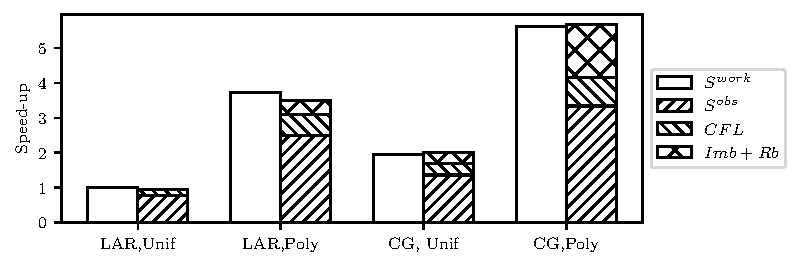
\includegraphics{{adaptive_local_timestepping/images/bar_plot_speed_ups}.pdf}
\caption{Comparison of speed-up due to work  reduction $S^{work}$ against observed speed-up $S^{obs}$ and the impact of avoiding CFL computations $(CFL)$ and fixing load imbalance and rollbacks $(Imb + Rb)$ for the lake at rest (LAR) and Carrier-Greenspan (CG) problem on the uniform (Unif) and polynomial meshes (Poly).}
\label{fig:imbalance-bars}
\end{figure}

To distinguish between algorithmic overhead of computing the CFL condition and other performance issues, we account for the cost of the CFL condition by multiplying the MPI execution times by the ratio of the execution times between the CFL and the no-CFL configurations of the lake at rest problem on the uniform mesh using the Devastator runtime. With these corrections, we obtain \effLARPoly{} of $S^{work}$ for the lake at rest problem with the polynomial mesh, \effCGUnif{} of $S^{work}$ of the Carrier-Greenspan problem with the uniform mesh, and \effCGPoly{} of $S^{work}$ of the Carrier-Greenspan problem for the polynomial mesh.
Furthermore, the impact of load imbalance and rollbacks is approximated by considering the average imbalance during the simulation. The imbalance is computed as the ratio of cells updated (both rolled back and committed) on the most overworked rank divided by the average number of committed cell updates across all ranks. Over a sufficiently small time interval this imbalance ratio approximates the improvement obtained through perfect load balancing. We estimate the impact of load imbalance by considering average imbalance over 100 evenly sized time intervals.

The cumulative performance impacts of the CFL computation and load imbalance are shown in Figure~\ref{fig:imbalance-bars}. This graph compares the speed-up due to work reduction, $S^{work}$ against the observed speed-up $S^{obs}$ and illustrates how the CFL computation and load imbalance account for the discrepancy. It is important to note that a given part of the stacked bar graph multiplies factors below it, e.g. the top of the $Imb+Rb$ bar corresponds to the expected speed-up if the simulation were perfectly balanced {\em and} there was no cost associated with the CFL condition. This distorts the size of bars towards the top of the graph, but allows us to compare the magnitudes of the speed-ups across problem configurations. With these two factors, we are able to account for the discrepancy in expected $S^{work}$ and observed $S^{obs}$ speed-ups within $\maxSpeedupErr\%$.

We also observed that rollback had a limited impact on performance for our experimental configurations.  For the Carrier-Greenspan problem, rollback minimally impacted the imbalance of the simulation with the imbalance metric increasing by no more than \imbCGdtRb{} for either mesh. For the polynomial lake at rest problem, the imbalance of committed updates was only \polynomialImb . However, once rollbacks are taken into consideration the imbalance went up to \polynomialImbwRb . Rollbacks are observed near regions of large CFL variation. For the Carrier-Greenspan problem, the lack of local clustering in the mapping of submeshes to ranks distributed rollbacks across ranks, and the impact of rollbacks on imbalance is relatively limited. However, for the polynomial lake at rest problem, each rank is assigned a contiguous chunk of submeshes, and rollback tends to aggregate on a few ranks.

Another cause of the performance degradation due to imbalance may be limitations of static load balancing. Firstly, there exist discrepancies between the performance model outlined in Section~\ref{sec:load-balancing} and the observed work done by each submesh, as evidenced by discrepancies between $S^{th}$ and $S^{work}$. Since the load balancing is based on the work of the theoretical model, this may lead to load imbalances, which we are not accounting for. Furthermore, the lower bound for the imbalance of the Carrier-Greenspan problem at the end of the Gurobi partitioning was 20\%. Although this lower bound does not account for the discrepancy between the performance model and observed work as well as error due to the quadrature used to approximate the integral in \eqref{eq:lb}, it suggests that there are underlying limits to how well the partitioner is able to statically load balance the problem. In that case, further reduction in load imbalance would benefit from dynamic load balancing techniques outlined in~\cite{Bremer2018}.

Lastly, we note that while the overhead associated with computing the CFL condition may seem high, it is worth noting that the MPI implementation is not provably stable. For the results presented here, we are able to take optimal timestep sizes, because we are able to analytically determine $(\Lambda / \delta x)_{\max}$. In practice, this value is unobtainable, and the selected $\Delta t$ would either lead to sub-optimal timestepping, i.e. taking timesteps smaller than necessary or manifest instabilities. The local timestepping algorithm can set an arbitrarily small $\Delta t_{\min}$,  and then take appropriately sized timesteps with step-size reductions taken as needed to guarantee stability.
 %2 pages

\section{Conclusion}

This work presented an adaptive local timestepping algorithm for conservation laws. Loop invariants were used to derive a proof of formal correctness, ensuring that the algorithm is total variation stable even when considering dynamic changes in local wave speeds. Furthermore, the algorithm was parallelized using a speculative parallel discrete event simulator. Results indicate that the parallelization recovers a majority of the expected speed-up, when accounting for the cost of the CFL condition.

As part of our future work, we will examine higher order timestepping strategies. The forward Euler step forms the basis of higher order strong stability preserving methods. Future work will include the development of higher order adaptive timestepping methods in the spirit of~\cite{Constantinescu2007}. Furthermore, we aim to apply this method to physically relevant coastal modeling problems to better quantify benefit of adaptive local timestepping to communities of interest.

At a more general level this work makes two important contributions to the development of asynchronous algorithms. Firstly, the nonlinearity of this problem makes knowing the task graph a priori impossible. While there has been an emergence of task-based runtimes in recent years to address architectural heterogeneity, this work calls into question the efficacy of a task-dependency graph as the sole means of representing scientific computing work flows within these modern runtime systems. Close interdisciplinary work is required with runtime system engineers and applied mathematicians to ensure that avenues for efficient implementations of adaptive algorithms remain accessible.

Secondly, the application of loop invariant analysis in order to assess the correctness of application significantly simplifies the development. Formal correctness techniques are expected to play an increasingly important role in the era of extreme heterogeneity as exhaustively replicating the states of a system in a highly concurrent setting will become increasingly difficult~\cite{ExtremeHeterogeneity2018}. The results here showcase how to use the invariant analysis proposed in~\cite{Bientinesi2011}. Due to the formal correctness proof, we ran into significantly fewer bugs during application development. Nevertheless, we found the derivation of the proof to be tedious. Automating this proof technique would allow us to better manage complexity and support the derivation of increasingly complicated algorithms.

 %1/2 page



%\begin{appendices}
% \crefalias{chapter}{appendix}

\singlespacing%
%\nocite{*}      % This command causes all items in the 		     %
%                % bibliographic database to be added to 	     %
%                % the bibliography, even if they are not 	     %
%                % explicitly cited in the text. 		     %
%\bibliographystyle{plain}  % Here the bibliography 		     %
\bibliographystyle{unsrt}  % Here the bibliography 		     %
\bibliography{BremerBib/Timestepping,BremerBib/HPC,BremerBib/DG,BremerBib/SWE,BremerBib/DES,BremerBib/LoadBalancing}
%\input{vita.tex}
%\end{appendices}

\end{document}

